\documentclass[11pt]{article}
\usepackage[margin=1in]{geometry}
\usepackage{newtxtext,newtxmath}
\usepackage{booktabs,graphicx,amsmath,caption,float}
\renewcommand{\topfraction}{0.9}
\renewcommand{\bottomfraction}{0.8}
\renewcommand{\textfraction}{0.07}
\renewcommand{\floatpagefraction}{0.75}
\usepackage[hidelinks]{hyperref}
\captionsetup{font=small}
\setlength{\parskip}{3pt}
\setlength{\emergencystretch}{2em}

\title{Assignment 1 Report}
\author{Name: Shirou Jing\\NetID: sj186}
\date{Oct.\ 20, 2026}

\begin{document}
\maketitle

\section{Experiment}

\textbf{Goal.} Part 1 implements a fully connected network in NumPy with hand-written backpropagation, first as the 3-layer network of the starter code and then as an $n$-layer network, and trains it on Make-Moons and on the scikit-learn Digits dataset. Part 2 trains the DCN conv(5-5-1-32)--ReLU--maxpool--conv(5-5-32-64)--ReLU--maxpool--fc(1024)--ReLU--dropout(0.5)--softmax(10) on MNIST in PyTorch, monitors weights, biases, net inputs and activations in TensorBoard, and compares activation functions, initializations and optimizers.

\section{Experiment Setup}

All experiments run on NERSC Perlmutter login nodes. Part 1 is NumPy on CPU; Part 2 runs on one A100 per run.

\begin{table}[H]
\centering
\caption{Environment.}
\begin{tabular}{ll}
\toprule
Item & Value \\
\midrule
System & NERSC Perlmutter, login node \\
GPU & NVIDIA A100-PCIE-40GB; driver 580.178.04 \\
CPU & AMD EPYC 7713 64-Core Processor \\
OS & SUSE Linux Enterprise Server 15 SP6 \\
Software & NERSC module \texttt{pytorch/2.13.0}: Python 3.12.13, PyTorch 2.13.0 (CUDA 13.0), \\
 & torchvision 0.28.0, NumPy 2.4.4, scikit-learn 1.9.0, TensorBoard 2.21.0 \\
\bottomrule
\end{tabular}
\end{table}

\section{Results and Discussion}

\subsection{Make-Moons Dataset}

\texttt{generate\_data()} draws 200 points from \texttt{make\_moons} with noise 0.2 (Figure~\ref{fig:moons}). The two classes interleave, so no linear boundary separates them.

\begin{figure}[tbp]
\centering
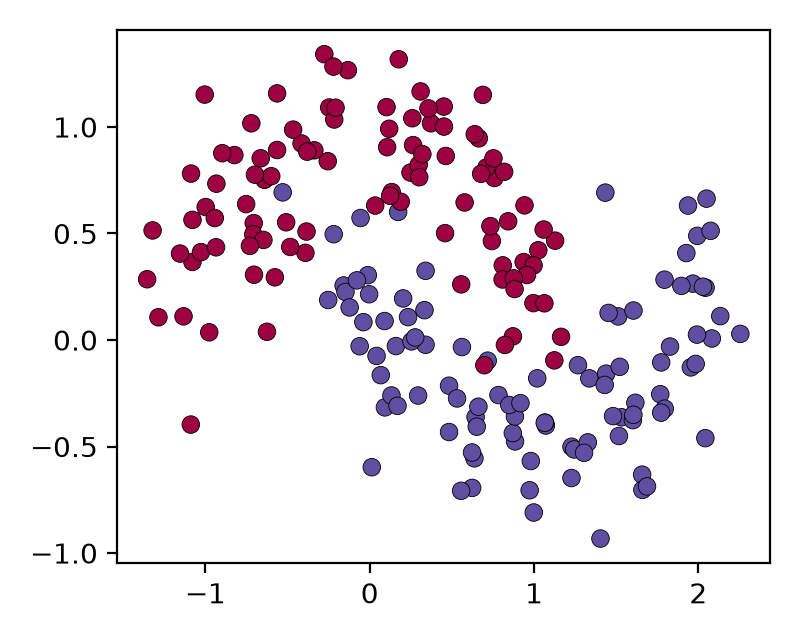
\includegraphics[width=0.34\linewidth]{figures/p1a_moons.png}
\caption{Make-Moons, 200 samples, noise 0.2.}
\label{fig:moons}
\end{figure}

\subsection{Activation Functions and Their Derivatives}

With $\sigma(z)=1/(1+e^{-z})$:
\begin{align*}
\frac{d}{dz}\tanh z &= \frac{(e^{z}+e^{-z})^2-(e^{z}-e^{-z})^2}{(e^{z}+e^{-z})^2} = 1-\tanh^2 z,\\
\frac{d}{dz}\sigma(z) &= \frac{e^{-z}}{(1+e^{-z})^2} = \sigma(z)\bigl(1-\sigma(z)\bigr),\\
\frac{d}{dz}\max(0,z) &= \begin{cases}1 & z>0\\ 0 & z<0\end{cases}
\end{align*}
The ReLU derivative is undefined at $z=0$; the code uses 0 there. \texttt{actFun} and \texttt{diff\_actFun} implement these expressions directly.

\subsection{Forward Pass and Loss}

Samples are stacked as rows of $X\in\mathbb{R}^{N\times 2}$, so the code computes $z_1=XW_1+b_1$, $a_1=f(z_1)$, $z_2=a_1W_2+b_2$ and $\hat Y=\mathrm{softmax}(z_2)$ row-wise, which is Eqs.~(1)--(4) transposed. The softmax subtracts the row maximum before exponentiating. \texttt{calculate\_loss} returns Eq.~(5) plus the starter code's L2 term:
\[
L=-\frac1N\sum_{n}\log \hat y_{n,y_n}+\frac{\lambda}{2N}\bigl(\|W_1\|^2+\|W_2\|^2\bigr).
\]

\subsection{Backpropagation}

For one sample, $\partial \hat y_j/\partial z_{2,k}=\hat y_j(\delta_{jk}-\hat y_k)$, so
\[
\frac{\partial}{\partial z_{2,k}}\Bigl(-\sum_j y_j\log\hat y_j\Bigr)=-\sum_j y_j(\delta_{jk}-\hat y_k)=\hat y_k-y_k,
\]
using $\sum_j y_j=1$. Over the batch, $\delta_2\equiv\partial L/\partial z_2=\frac1N(\hat Y-Y)$. The chain rule then gives
\begin{align*}
\frac{\partial L}{\partial W_2} &= a_1^\top\delta_2+\frac{\lambda}{N}W_2, & \frac{\partial L}{\partial b_2} &= \mathbf 1^\top\delta_2,\\
\delta_1\equiv\frac{\partial L}{\partial z_1} &= \bigl(\delta_2W_2^\top\bigr)\odot f'(z_1), &&\\
\frac{\partial L}{\partial W_1} &= X^\top\delta_1+\frac{\lambda}{N}W_1, & \frac{\partial L}{\partial b_1} &= \mathbf 1^\top\delta_1.
\end{align*}
\texttt{backprop} returns these gradients multiplied by $N$, i.e.\ summed over samples, and \texttt{fit\_model} adds $\lambda W$. This matches the starter's update rule, and the learning rate $\epsilon=0.01$ absorbs the factor $N$. Against central finite differences, the maximum absolute gradient error is below $10^{-8}$ for all three activations.

\subsection{Training with Tanh, Sigmoid and ReLU}

Each network has 3 hidden units and is trained with the starter's settings: full-batch gradient descent, $\epsilon=0.01$, $\lambda=0.01$, 20{,}000 passes (Figure~\ref{fig:e1}). Test accuracy is measured on 2{,}000 fresh Make-Moons samples (noise 0.2, seed 1) that are never used for training.

\begin{figure}[tbp]
\centering
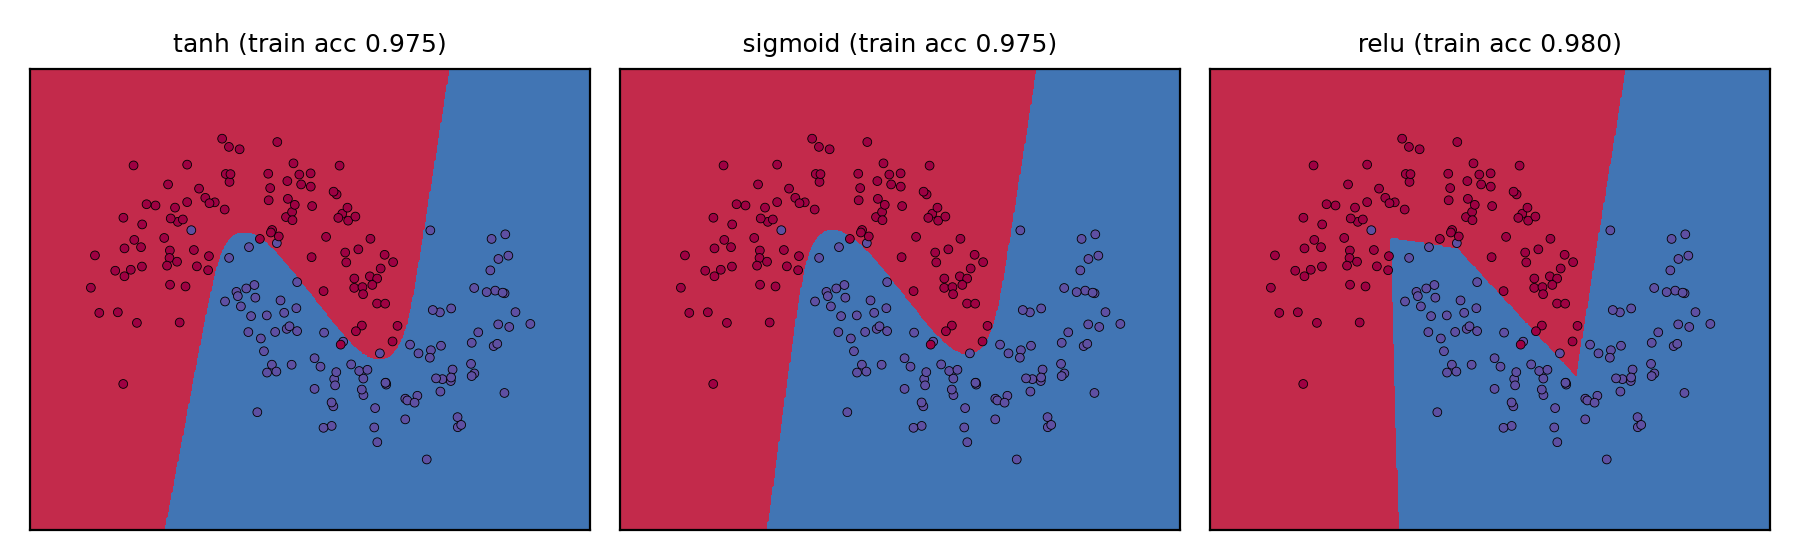
\includegraphics[width=\linewidth]{figures/p1e1_activations.png}
\caption{Decision boundaries, 3 hidden units. Test accuracy: tanh 0.967, sigmoid 0.967, ReLU 0.963.}
\label{fig:e1}
\end{figure}

All three reach 97.5--98\% training accuracy, and the shapes of the boundaries differ. Tanh and sigmoid give smooth curves. Sigmoid is a shifted and rescaled tanh, $\sigma(z)=\tfrac12(1+\tanh\tfrac z2)$, so with enough training the two networks represent the same function family; sigmoid ends at a slightly higher loss (0.078 vs.\ 0.071). Its derivative is at most 0.25, against 1 for tanh, so with the same step size it moves more slowly. The ReLU boundary is piecewise linear with visible kinks: each hidden unit splits the plane along a line, and three units allow only a few linear pieces.

\subsection{Number of Hidden Units}

Tanh networks with 1--50 hidden units, same settings (Figure~\ref{fig:e2}).

\begin{figure}[tbp]
\centering
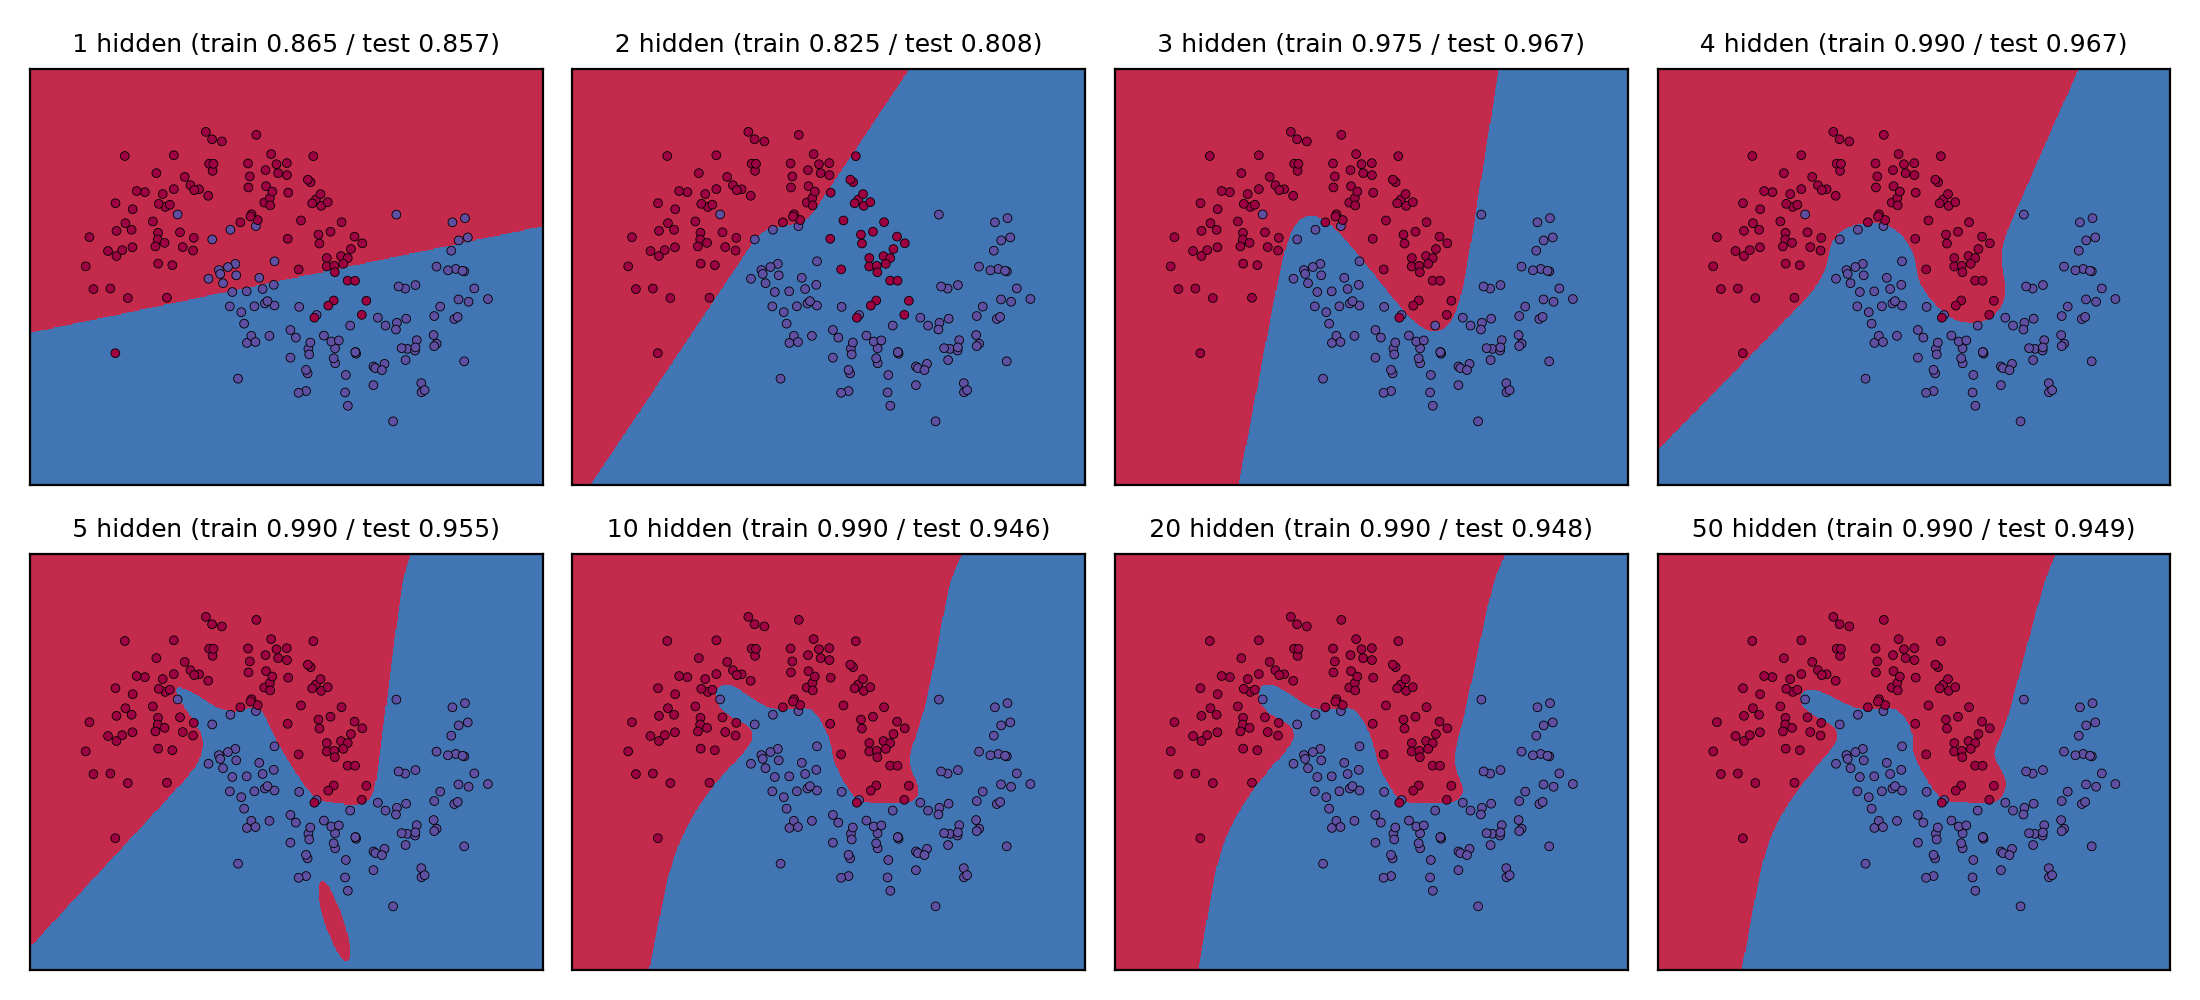
\includegraphics[width=\linewidth]{figures/p1e2_hidden.png}
\caption{Tanh, varying hidden width.}
\label{fig:e2}
\end{figure}

With 1 or 2 units the boundary is close to a line (train 0.865/0.825). Three units are enough to bend around both moons, and test accuracy is highest at 3--4 units (0.967). Beyond that, training accuracy saturates at 0.99 and the extra capacity goes into fitting individual noisy points. At 5 units an isolated island appears around a single sample; at 10--50 units the boundary curls around the outliers in the middle. Test accuracy falls to 0.946--0.955. The $\lambda=0.01$ penalty is weak relative to the summed data loss, so it does not prevent this.

\subsection{Deep Network Implementation}

\texttt{n\_layer\_neural\_network.py} follows the hints. \texttt{Layer} stores $W$, $b$ and its forward cache ($x$, $z$) and implements \texttt{feedforward(x, actFun)} and \texttt{backprop(da, diff\_actFun)}. The backward method returns $\partial L/\partial x$ for the layer below and stores $dW$ and $db$. \texttt{DeepNeuralNetwork} subclasses \texttt{NeuralNetwork} and reuses its \texttt{actFun}, \texttt{diff\_actFun}, \texttt{predict} and plotting. The constructor takes \texttt{n\_layers} (counting input and output, so 3 is the network above) and \texttt{layer\_size}, which is either an integer for equal widths or a list of per-layer widths. Two choices differ from the 3-layer code:
\begin{itemize}\setlength\itemsep{0pt}
\item The loss averages over samples, $L=\frac1N\sum_n \mathrm{CE}_n+\frac\lambda2\sum_\ell\|W_\ell\|^2$, and the gradients are true gradients of $L$. The step size then does not depend on $N$, so the same $\epsilon$ works for 200 Moons points and 1{,}347 Digits samples. I use $\epsilon=0.1$ and $\lambda=10^{-3}$; with $\epsilon=1.0$ the 10-layer ReLU network fails to train.
\item The output layer is a \texttt{Layer} with identity activation, and softmax is applied in the network, so every layer shares one backward rule. Initialization stays $\mathcal N(0,1/\text{fan-in})$ as in the starter.
\end{itemize}
The finite-difference check from Section~3.4 also passes for a 5-layer network (maximum error $\sim10^{-10}$).

\subsection{Deep Networks on Make-Moons}

Figure~\ref{fig:depth} varies depth (3, 4, 6, 10 layers, width 10) and activation; Figure~\ref{fig:width} varies width at depth 6 with tanh. All runs use 20{,}000 passes.

\begin{figure}[tbp]
\centering
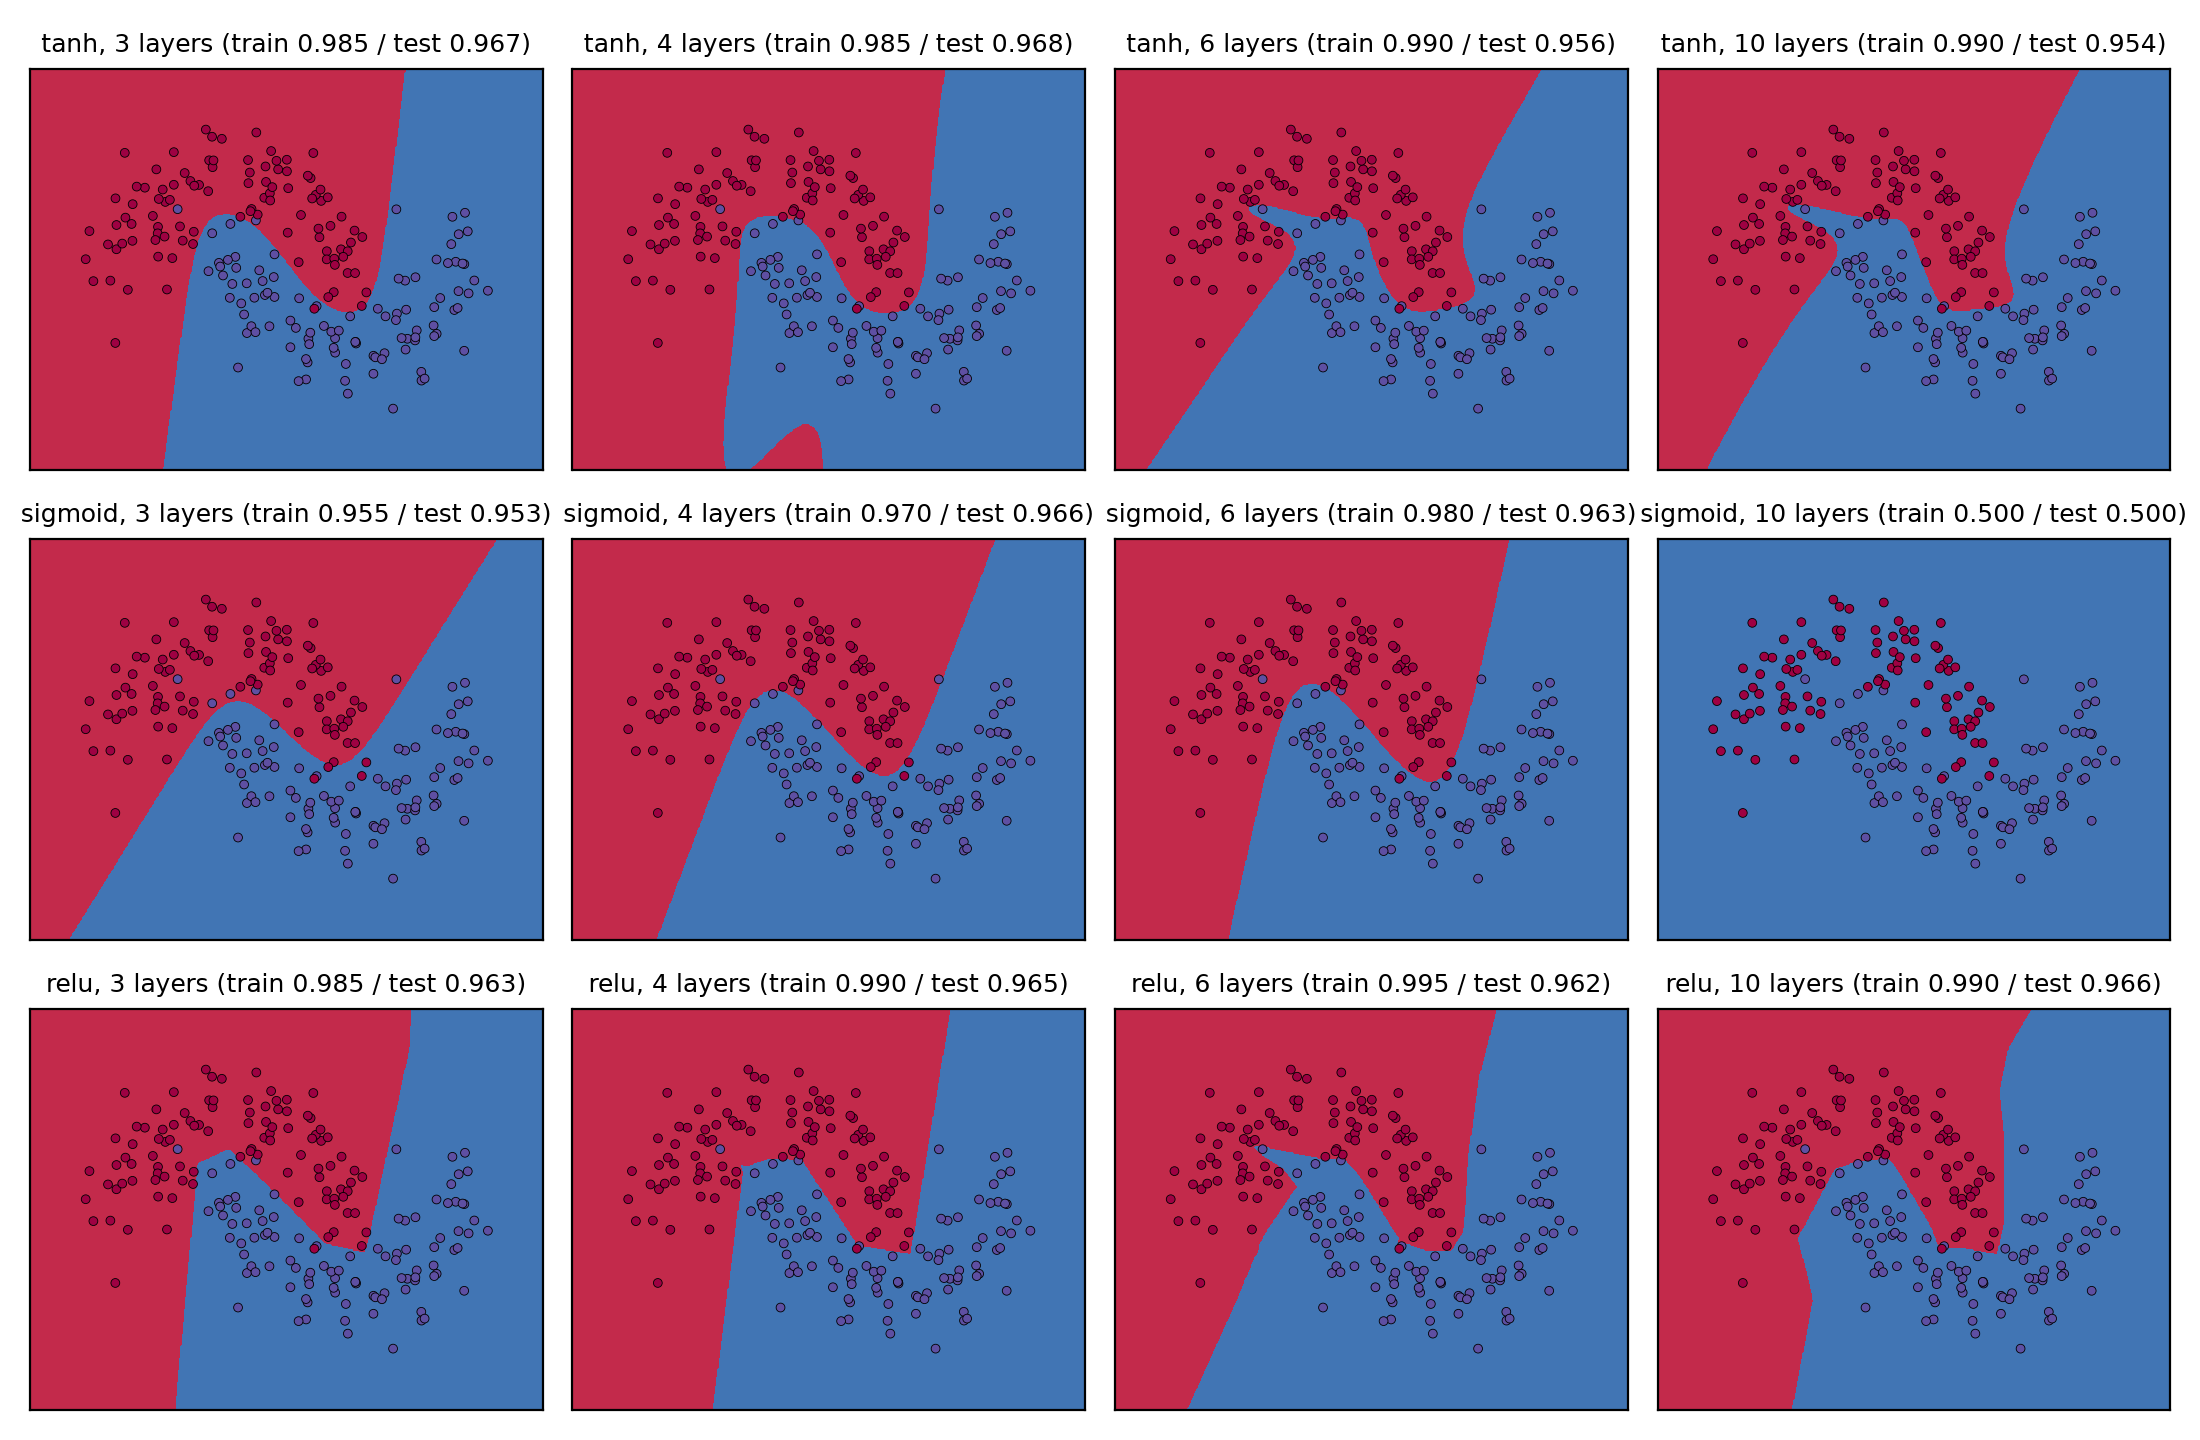
\includegraphics[width=\linewidth]{figures/p1f_depth.png}
\caption{Depth $\times$ activation, hidden width 10. Titles give train / test accuracy.}
\label{fig:depth}
\end{figure}

\begin{figure}[tbp]
\centering
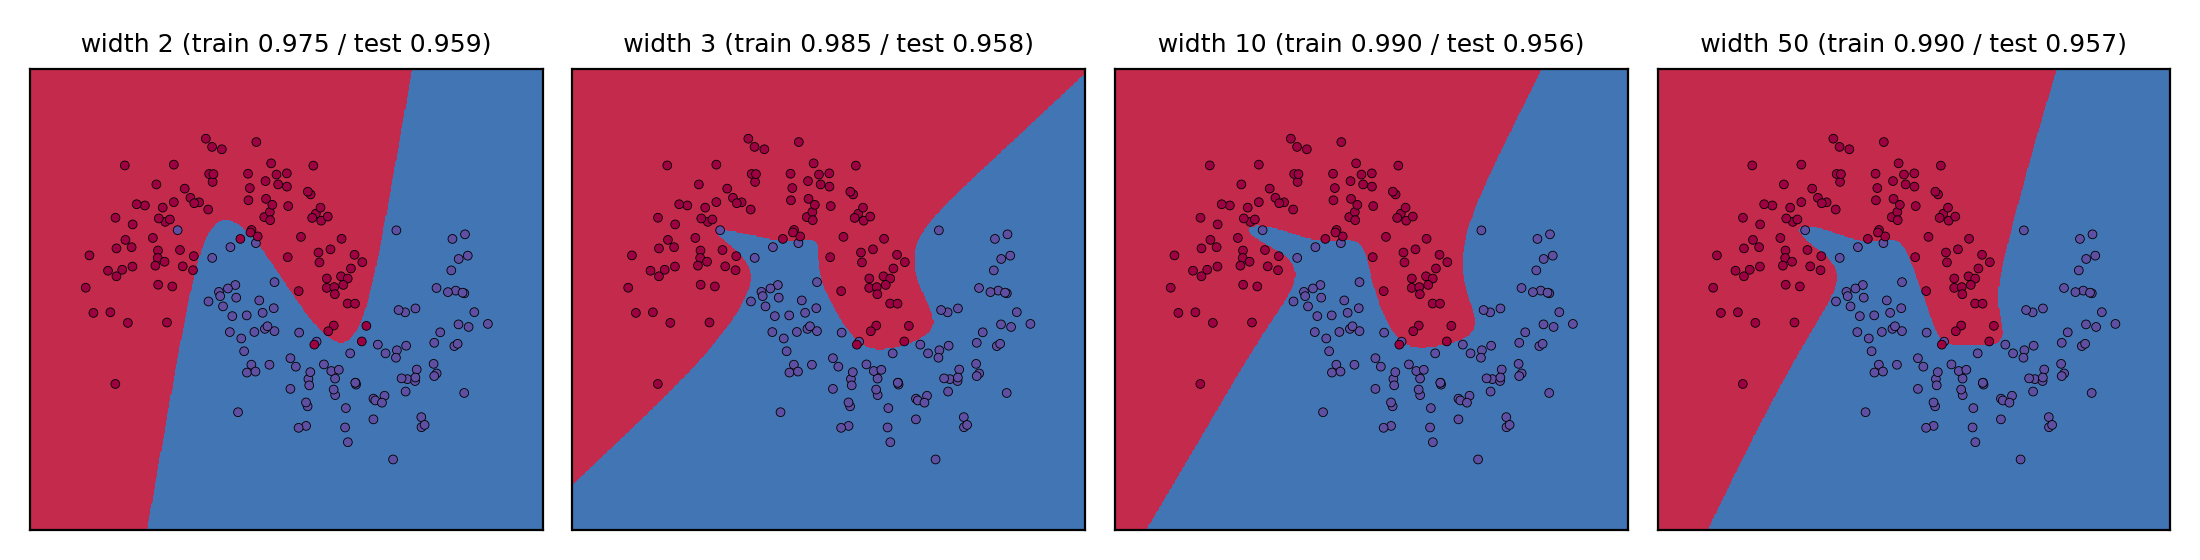
\includegraphics[width=\linewidth]{figures/p1f_width.png}
\caption{Width at 6 layers, tanh.}
\label{fig:width}
\end{figure}

Shallow networks draw one smooth S-curve. Deeper tanh and ReLU networks produce sharper, more folded boundaries, with narrow protrusions that reach into the other class to capture single points. Training loss falls from 0.116 (3 layers) to 0.045 (10 layers) for tanh, while test accuracy drops from 0.967 to 0.954, so the extra depth mostly fits noise. ReLU boundaries stay polygonal at every depth, and the number of linear pieces grows with depth. The sigmoid network with 10 layers does not train: it predicts one class everywhere and stays at loss 0.694, about $\ln 2$. Each sigmoid layer multiplies the backward signal by $\sigma'\le 0.25$, so across eight hidden layers the derivative factors alone shrink it by up to $0.25^8\approx 1.5\times10^{-5}$, and the first layers barely move. Tanh and ReLU at the same depth train normally. Width has a smaller effect than depth here. Width 2 already reaches 0.975 training accuracy at 6 layers, widths 10 and 50 give nearly the same boundary, and test accuracy stays at 0.956--0.959 for all widths.

\subsection{Deep Networks on Digits}

The second dataset is scikit-learn Digits: 1{,}797 grayscale $8\times8$ handwritten digits, 10 classes. The network has 64 inputs and 10 outputs. I use a stratified 75/25 split (1{,}347 / 450), standardize the features with training-set statistics, and run 5{,}000 full-batch passes with $\epsilon=0.1$ and $\lambda=10^{-3}$ (Table~\ref{tab:digits}, Figure~\ref{fig:digits}).

\begin{table}[H]
\centering
\caption{Digits test accuracy. Every tanh and ReLU network reaches 1.000 training accuracy.}
\label{tab:digits}
\begin{tabular}{lcccccc}
\toprule
 & \multicolumn{2}{c}{3 layers} & \multicolumn{2}{c}{4 layers} & \multicolumn{2}{c}{6 layers}\\
\cmidrule(lr){2-3}\cmidrule(lr){4-5}\cmidrule(lr){6-7}
Activation & 32 & 128 & 32 & 128 & 32 & 128\\
\midrule
tanh & 0.980 & 0.978 & 0.978 & 0.969 & 0.980 & 0.976\\
sigmoid & 0.976 & 0.978 & 0.969 & 0.969 & 0.691 & 0.891\\
ReLU & 0.973 & 0.978 & 0.978 & 0.978 & 0.964 & 0.982\\
\bottomrule
\end{tabular}
\end{table}

\begin{figure}[tbp]
\centering
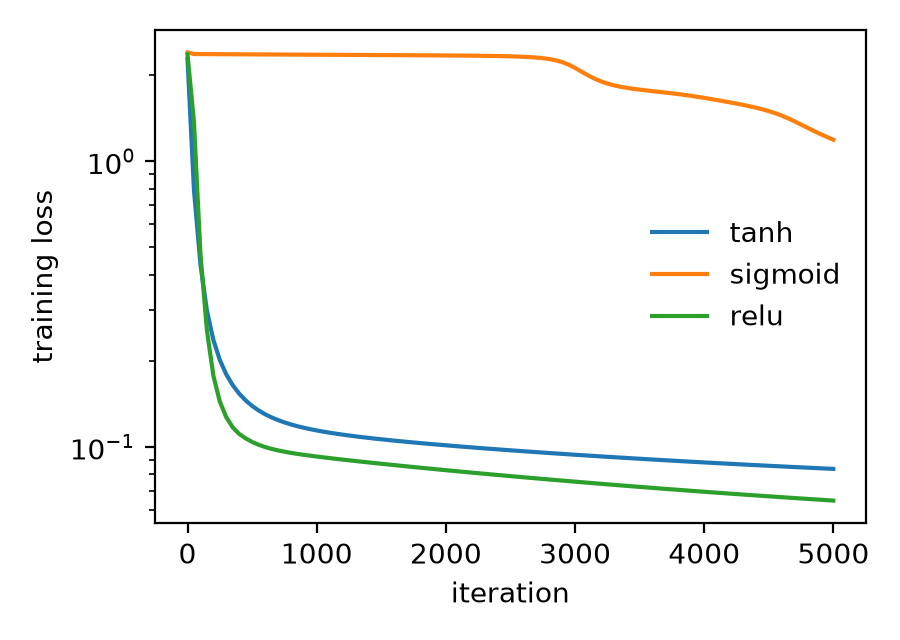
\includegraphics[width=0.48\linewidth]{figures/p1f_digits_loss.png}
\caption{Digits training loss, 6 layers, width 32.}
\label{fig:digits}
\end{figure}

A single hidden layer already gives 97--98\% test accuracy, and depth does not help: the classes are close to linearly separable in 64 dimensions, and with 1{,}347 samples every tanh and ReLU network fits the training set perfectly. With sigmoid at 6 layers and width 32, the loss stays on a plateau near $\ln 10$ for about 2{,}800 iterations before it starts to fall (Figure~\ref{fig:digits}), and after 5{,}000 passes it reaches only 70.6\% training and 69.1\% test accuracy. The plateau has the same cause as the 10-layer Moons failure: the backward signal shrinks through each sigmoid layer, so the early layers barely move until the later layers have organized. With width 128 the same depth gets further in 5{,}000 passes (89.1\% test). Tanh and ReLU leave the initial loss within 200 iterations.

\subsection{MNIST: Network and Training}

\texttt{mnist\_dcn.py} fills in the starter and keeps its structure. \texttt{Net} is conv(5$\times$5, 1$\to$32, padding 2)--\allowbreak ReLU--\allowbreak maxpool(2)--\allowbreak conv(5$\times$5, 32$\to$64, padding 2)--\allowbreak ReLU--\allowbreak maxpool(2)--\allowbreak fc(3136$\to$1024)--\allowbreak ReLU--\allowbreak dropout(0.5)--\allowbreak fc(1024$\to$10)--\allowbreak softmax. Padding 2 keeps $28\times28$ and $14\times14$ through the convolutions, as with SAME padding in the original tutorial. Training uses mini-batches of 64, the starter's loss \texttt{NLLLoss(log(softmax + 1e-13))}, and 10 epochs. The command-line flags \texttt{--act}, \texttt{--init}, \texttt{--opt} and \texttt{--lr} select the variants of Section~3.12. Two changes from the starter: the normalization mean is 0.1307, the MNIST pixel mean (the starter has 0.01307), and \texttt{torch.manual\_seed} is always called, because the starter seeds only CUDA while the weights are initialized on the CPU. The train loss is logged every 10 batches.

The starter's Adam learning rate of 0.01 does not train. After the first epoch every ReLU in conv2 and fc1 outputs zero on the monitoring batch, the network predicts a constant class, and test accuracy stays at chance level: 11.35\% (the share of the digit 1) in every epoch except epoch 8, where the prediction switches to the digit 8 (9.74\%). The baseline therefore uses Adam with lr $=10^{-3}$. It reaches 98.80\% test accuracy after one epoch and \textbf{99.17\%} after 10 epochs; the best epoch is 99.32\% (epoch 7). Figure~\ref{fig:a} shows the training loss: it falls from 2.30 to about 0.1 within the first few hundred iterations and keeps decreasing slowly after that.

\begin{figure}[tbp]
\centering
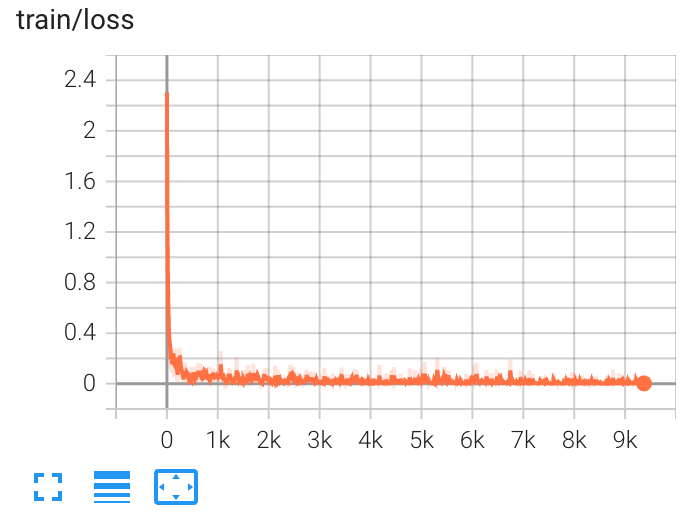
\includegraphics[width=0.45\linewidth]{screenshots/a_train_loss.png}
\caption{TensorBoard: training loss of the baseline (smoothing 0.6). The horizontal axis is iterations; 938 iterations make one epoch.}
\label{fig:a}
\end{figure}

\subsection{MNIST: Monitoring Weights, Activations and Test Error}

After every epoch, and once before training, the code logs min, max, mean, standard deviation and a histogram for:
\begin{itemize}\setlength\itemsep{0pt}
\item the weights and biases of all four layers;
\item the net inputs of conv1, conv2, fc1 and fc2;
\item the ReLU outputs of conv1, conv2 and fc1;
\item the max-pool outputs of both conv blocks.
\end{itemize}
Net inputs and activations are computed on a fixed batch of 1{,}000 test images in eval mode. Test loss, accuracy and error are logged every epoch. Figures~\ref{fig:btest}--\ref{fig:bstd} show the baseline. Figure~\ref{fig:bstats} gives all four statistics for two layers, and Figure~\ref{fig:bstd} gives the standard deviation of every monitored tensor.

\begin{figure}[tbp]
\centering
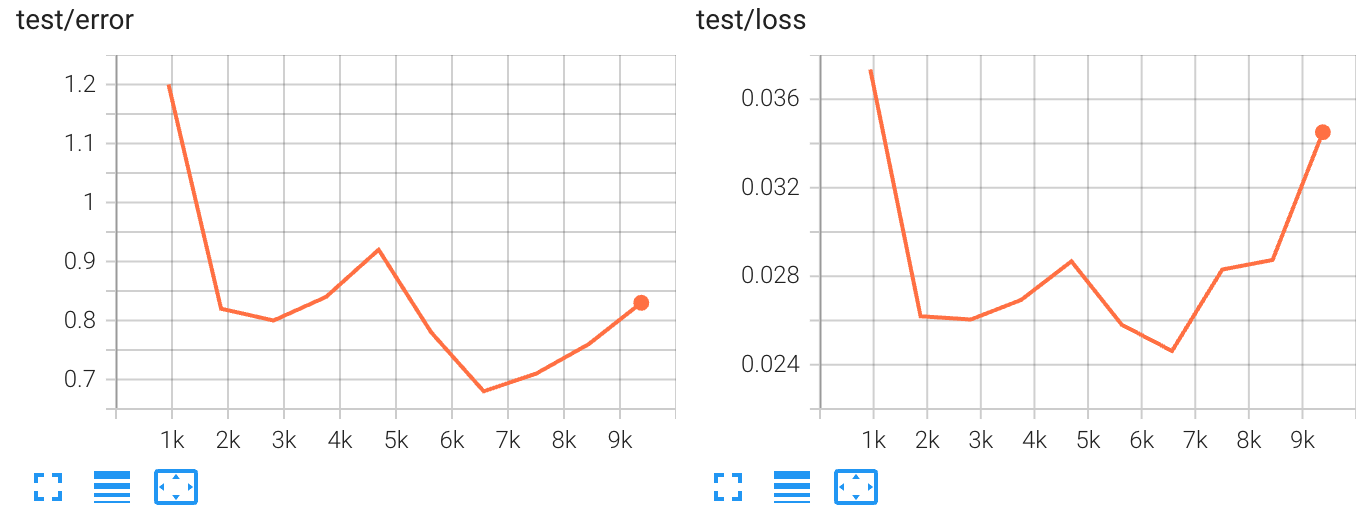
\includegraphics[width=0.6\linewidth]{screenshots/b_test.png}
\caption{Test error (\%) and test loss per epoch.}
\label{fig:btest}
\end{figure}

\begin{figure}[tbp]
\centering
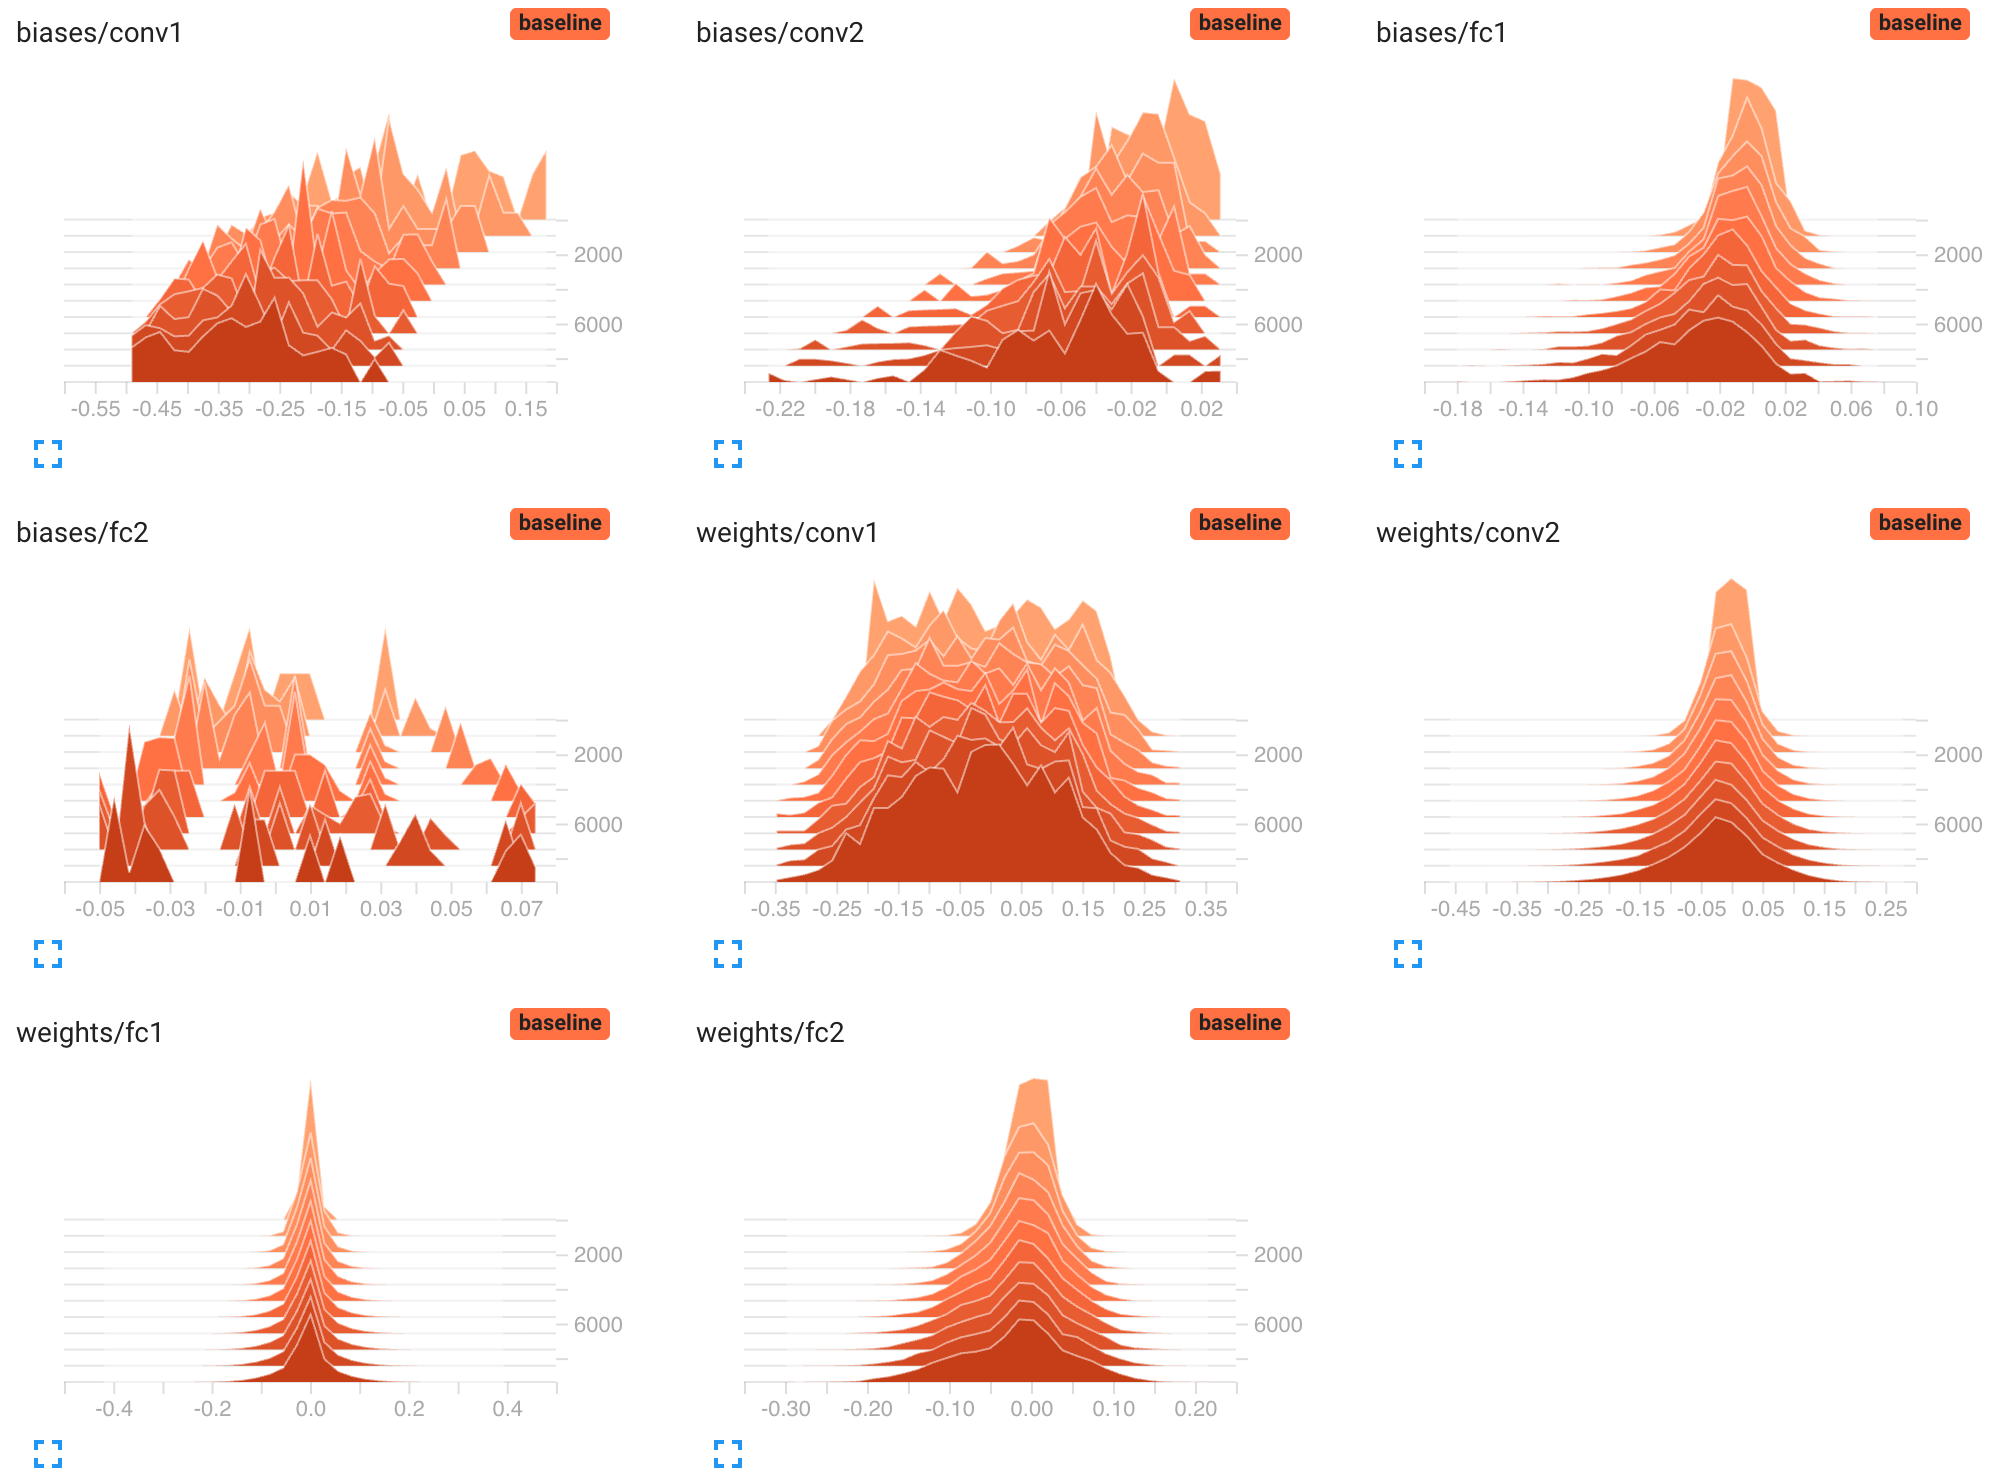
\includegraphics[width=0.72\linewidth]{screenshots/b_hist_params.png}
\caption{Histograms of biases and weights; front slices are later epochs.}
\label{fig:bhistp}
\end{figure}

\begin{figure}[tbp]
\centering
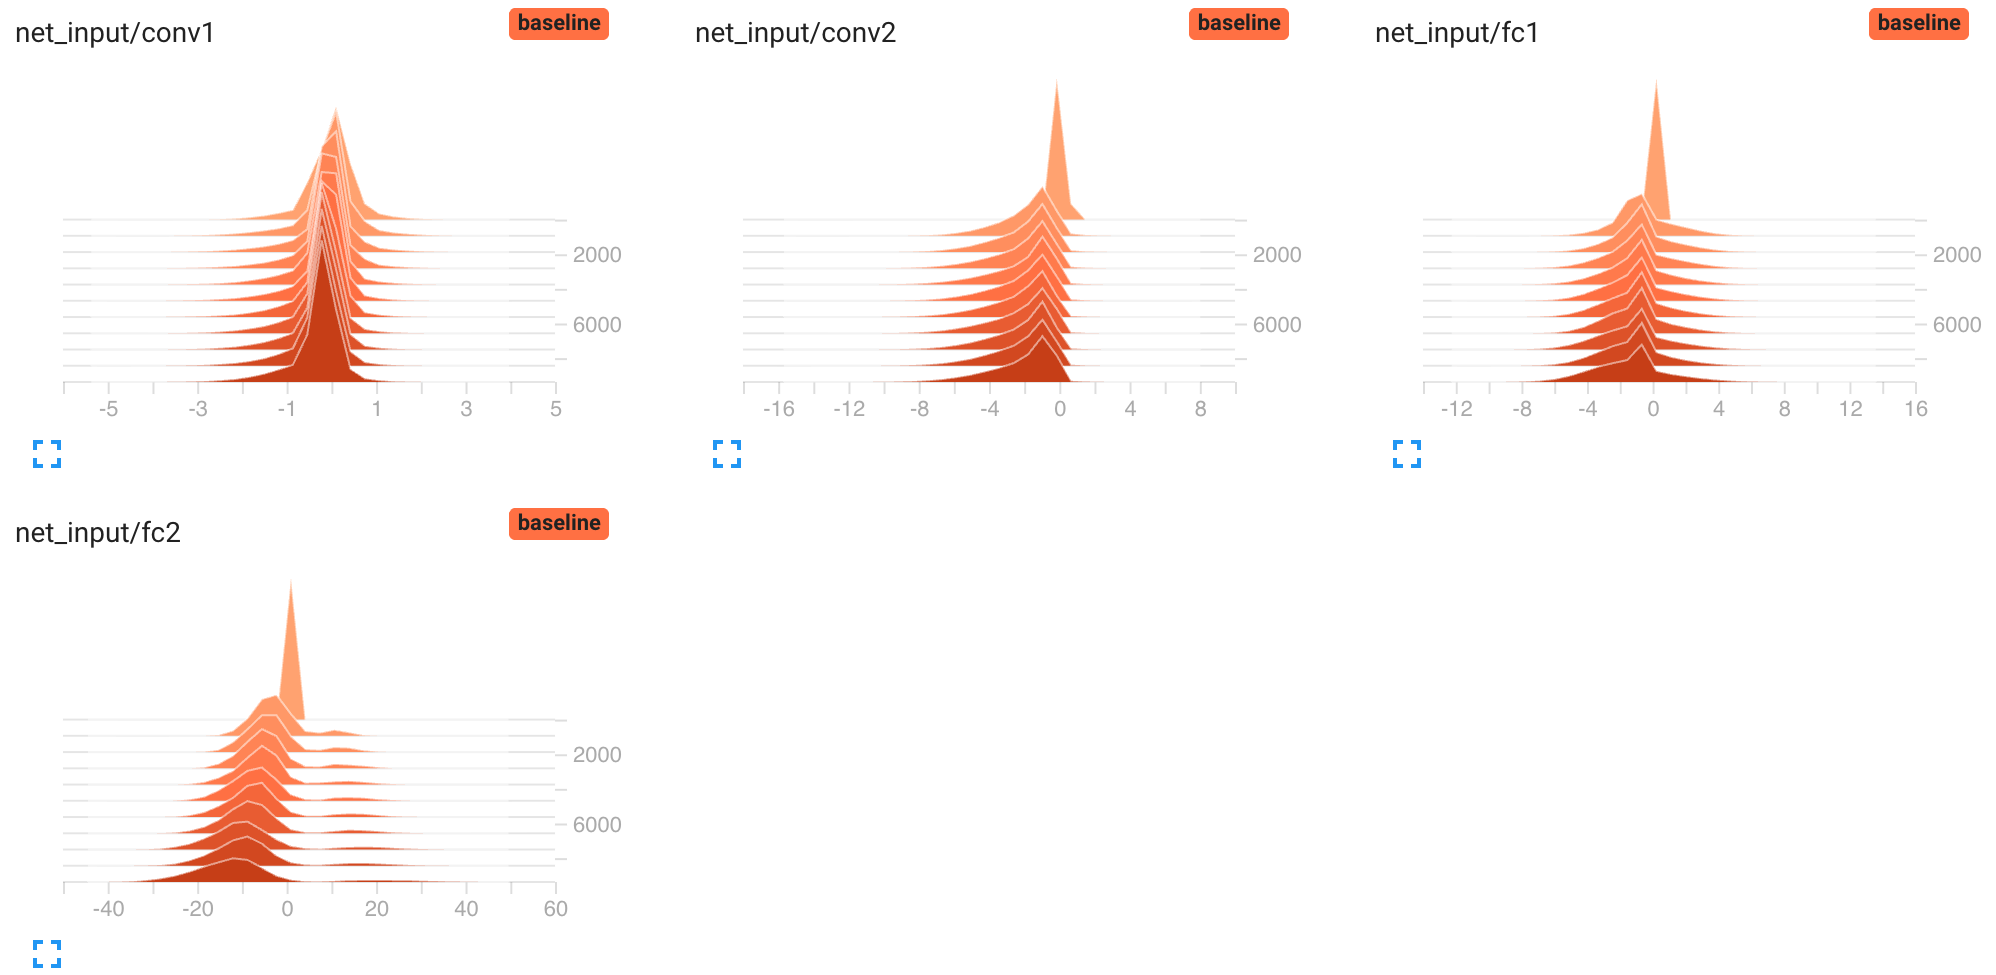
\includegraphics[width=0.66\linewidth]{screenshots/b_hist_netinput.png}

\vspace{4pt}
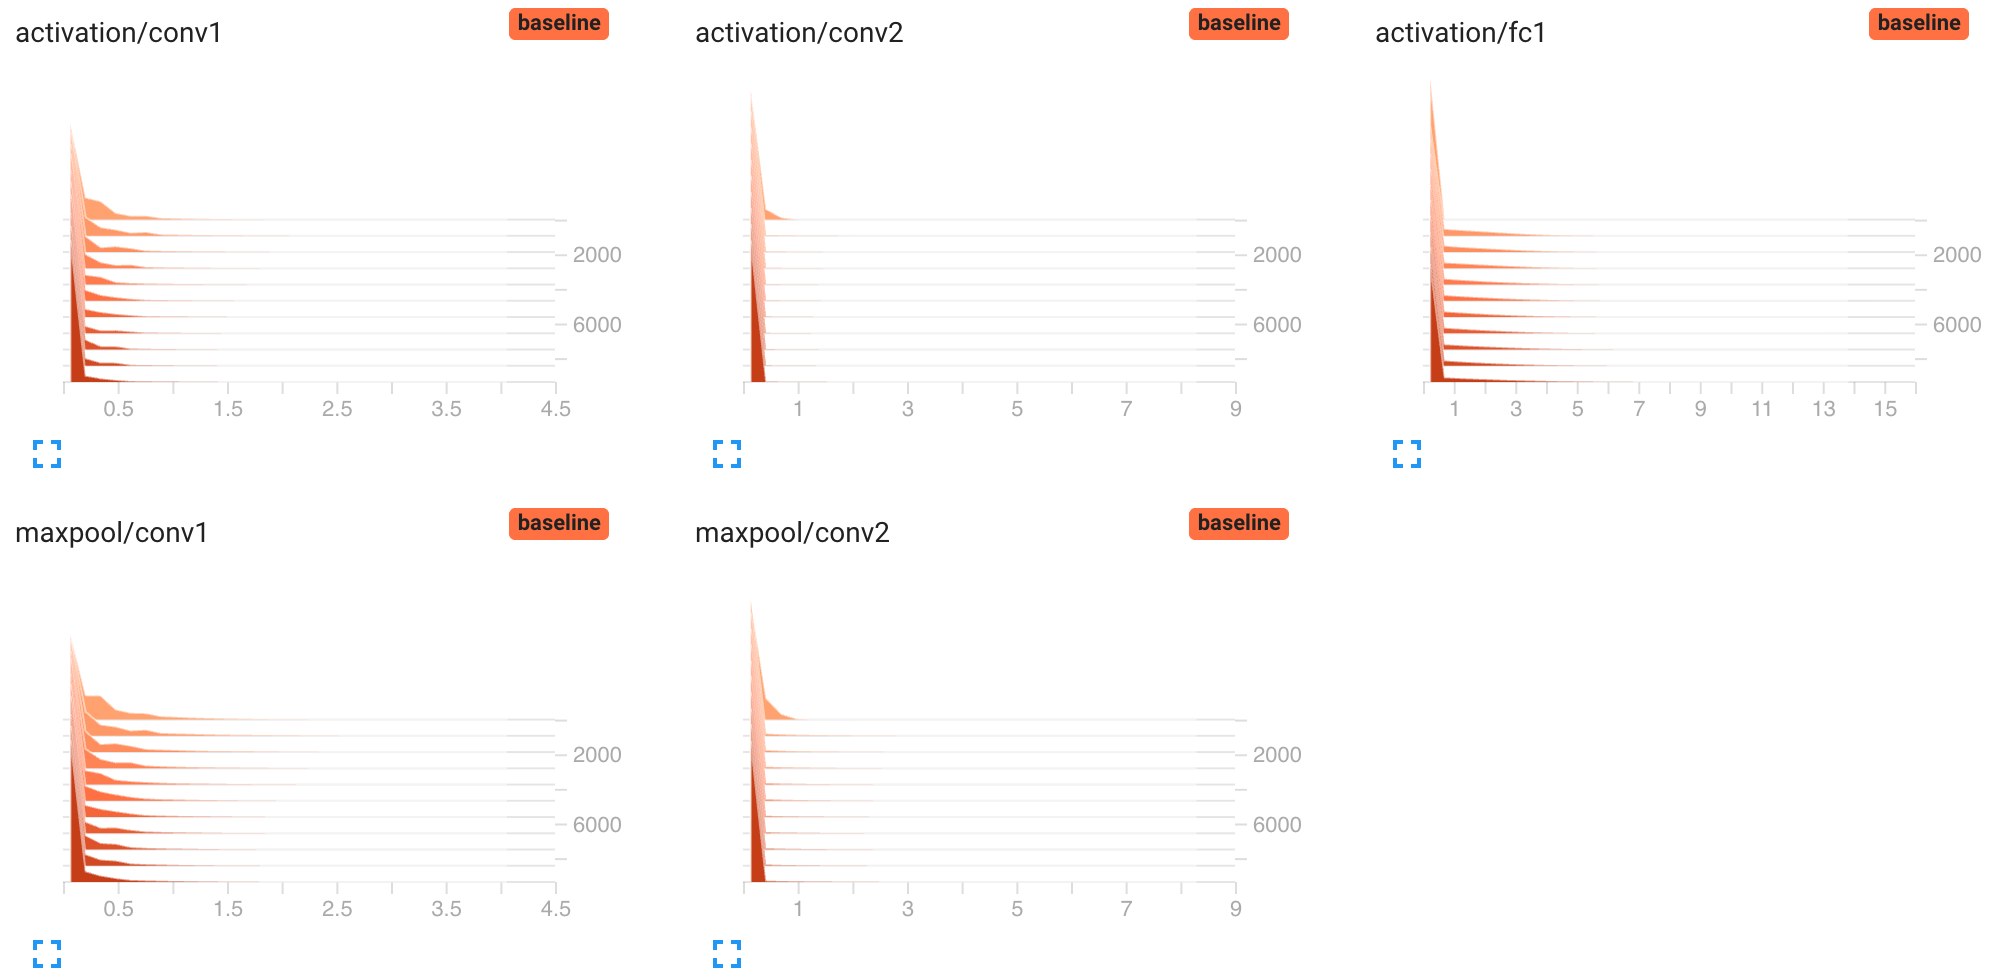
\includegraphics[width=0.66\linewidth]{screenshots/b_hist_act.png}
\caption{Histograms of net inputs (top), ReLU outputs and max-pool outputs (bottom).}
\label{fig:bhista}
\end{figure}

\begin{figure}[tbp]
\centering
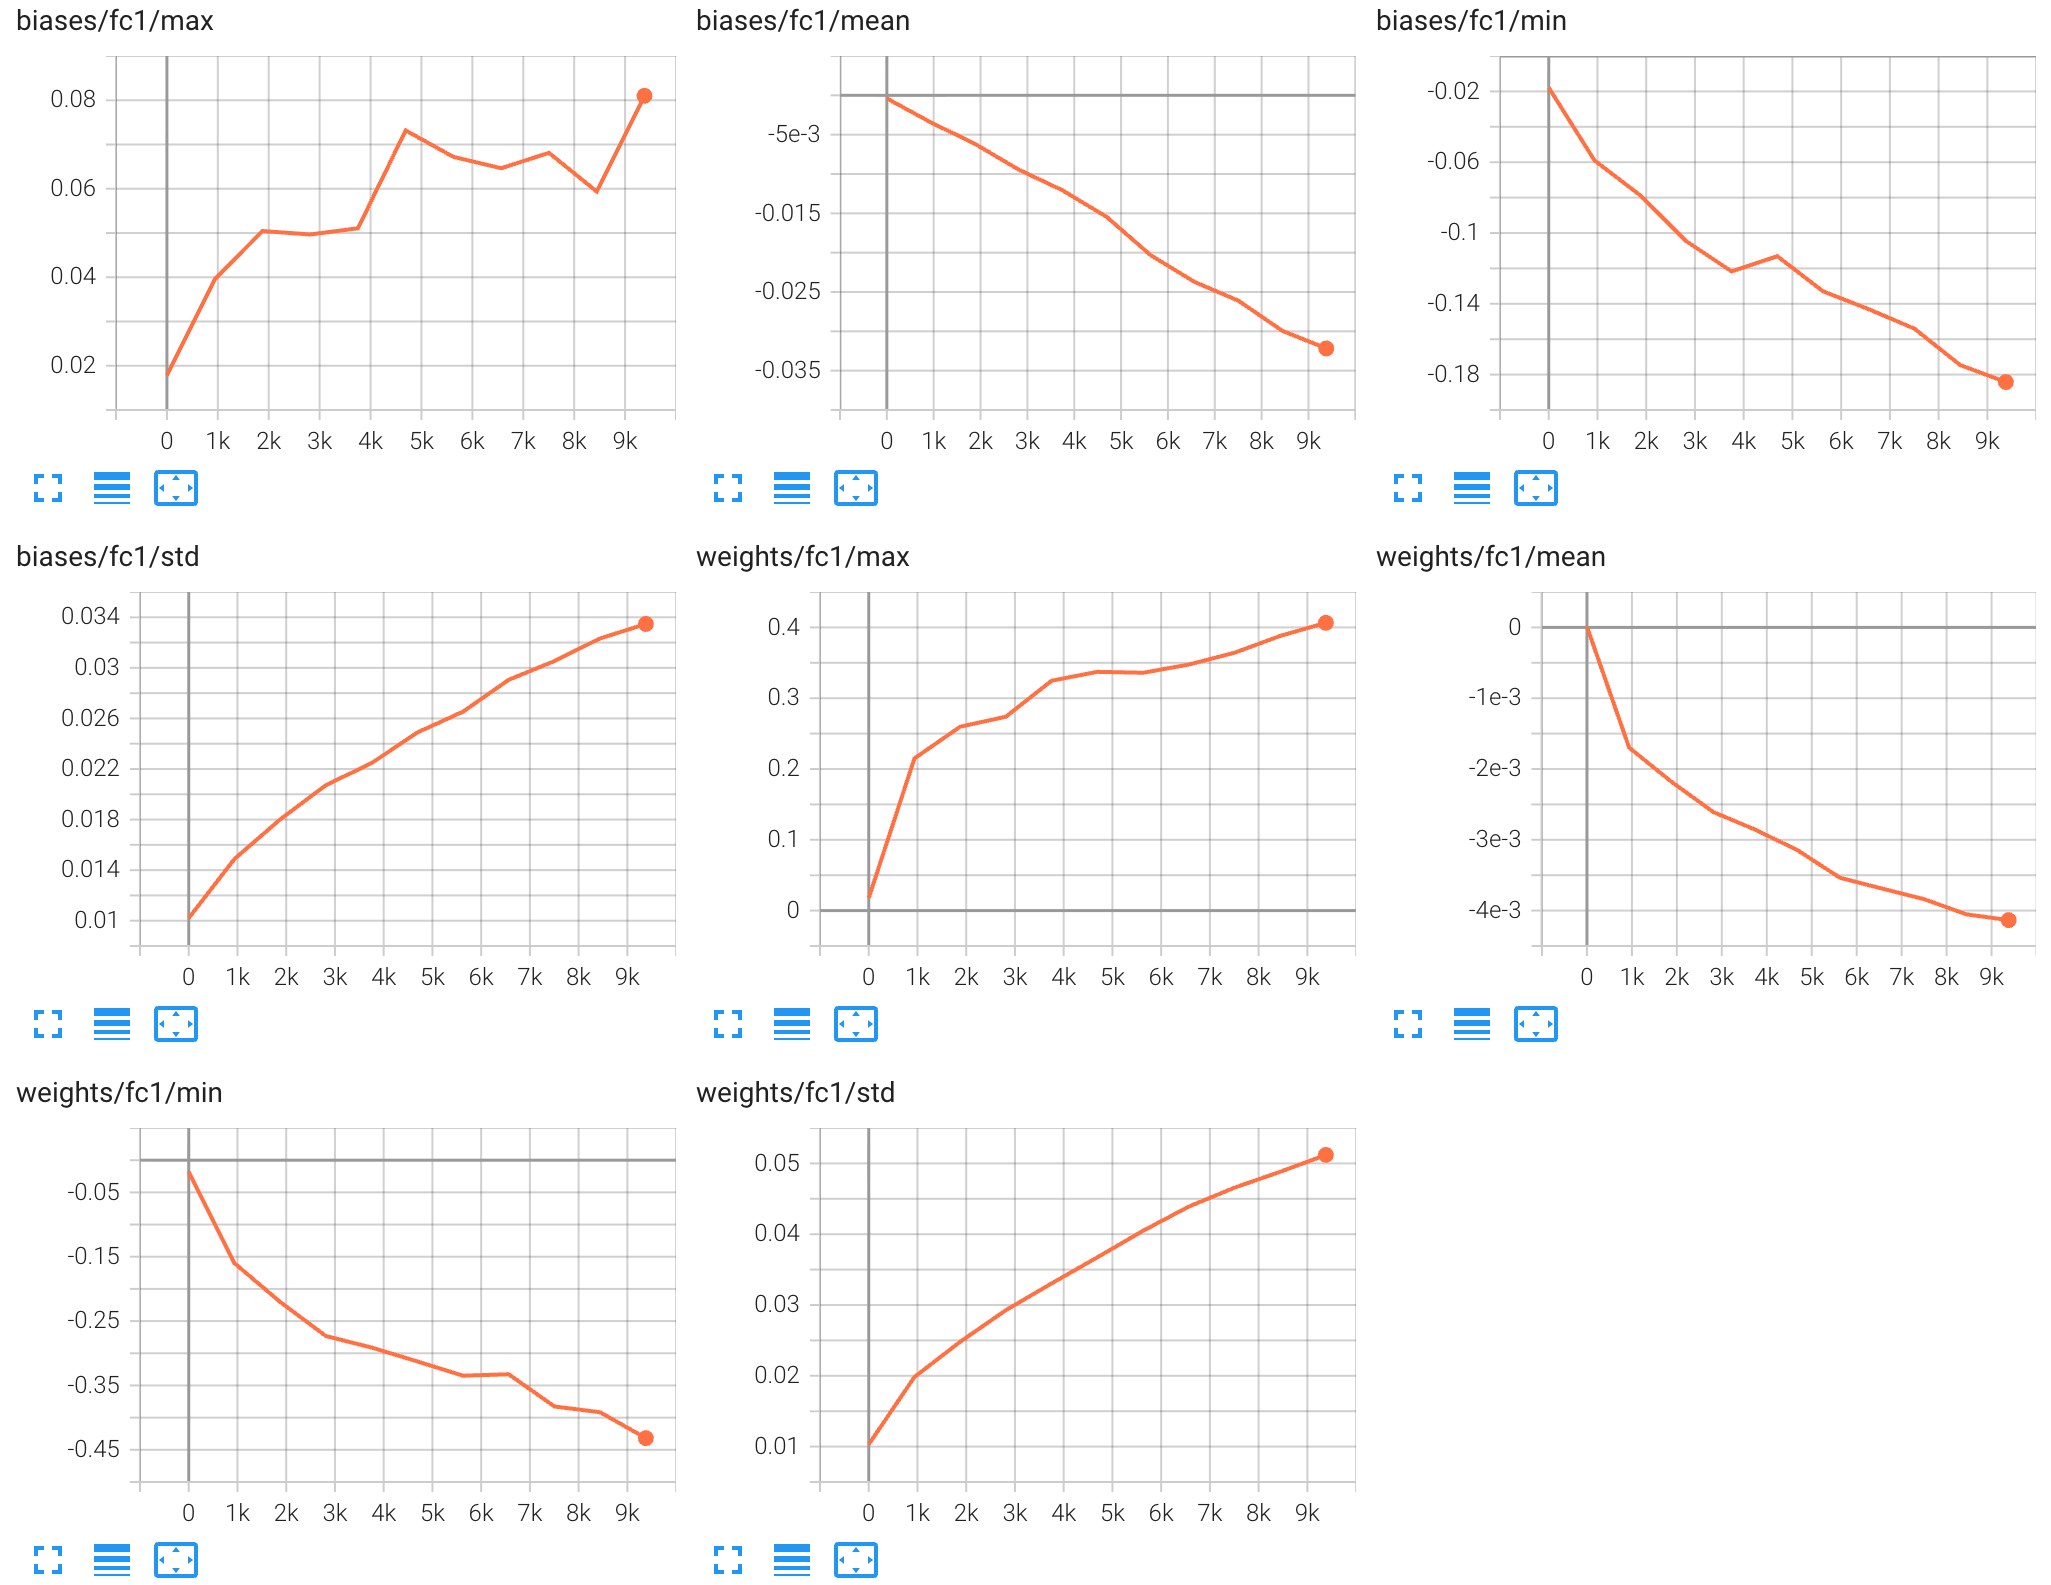
\includegraphics[width=0.62\linewidth]{screenshots/b_stats_params.png}

\vspace{4pt}
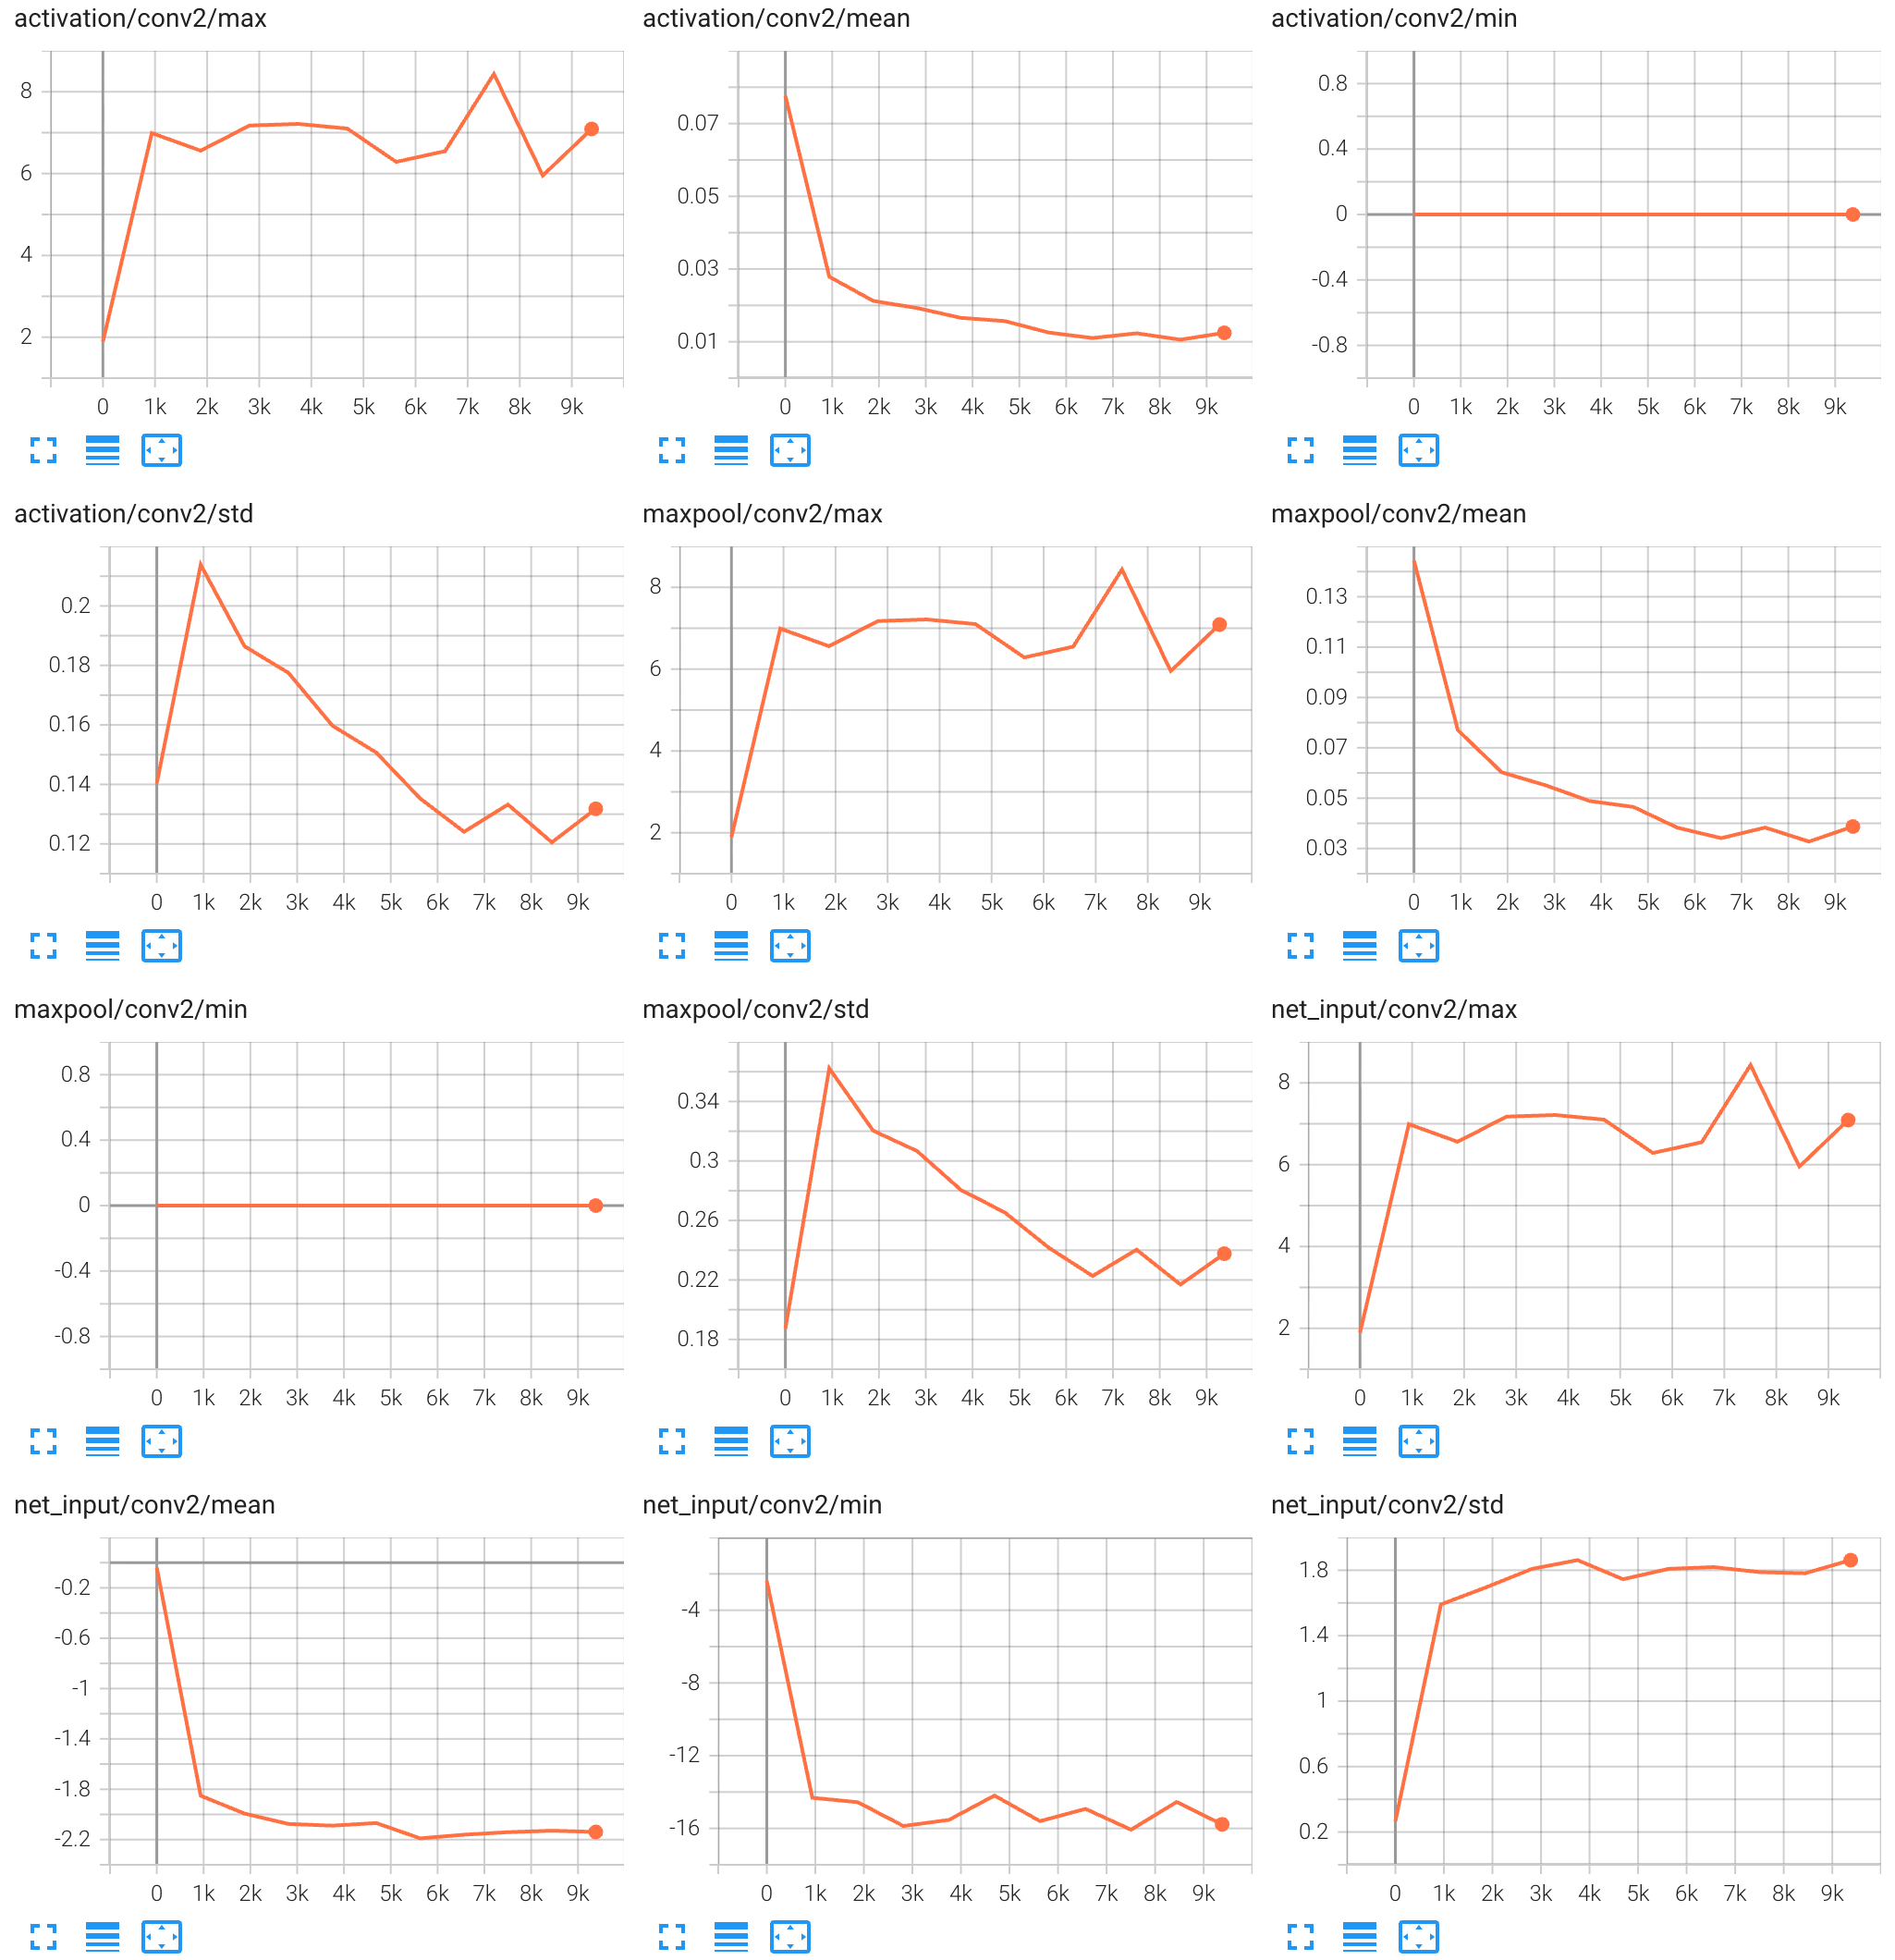
\includegraphics[width=0.62\linewidth]{screenshots/b_stats_conv2.png}
\caption{Min/max/mean/std of fc1 weights and biases (top) and of the conv2 net input, ReLU output and max-pool output (bottom).}
\label{fig:bstats}
\end{figure}

\begin{figure}[tbp]
\centering
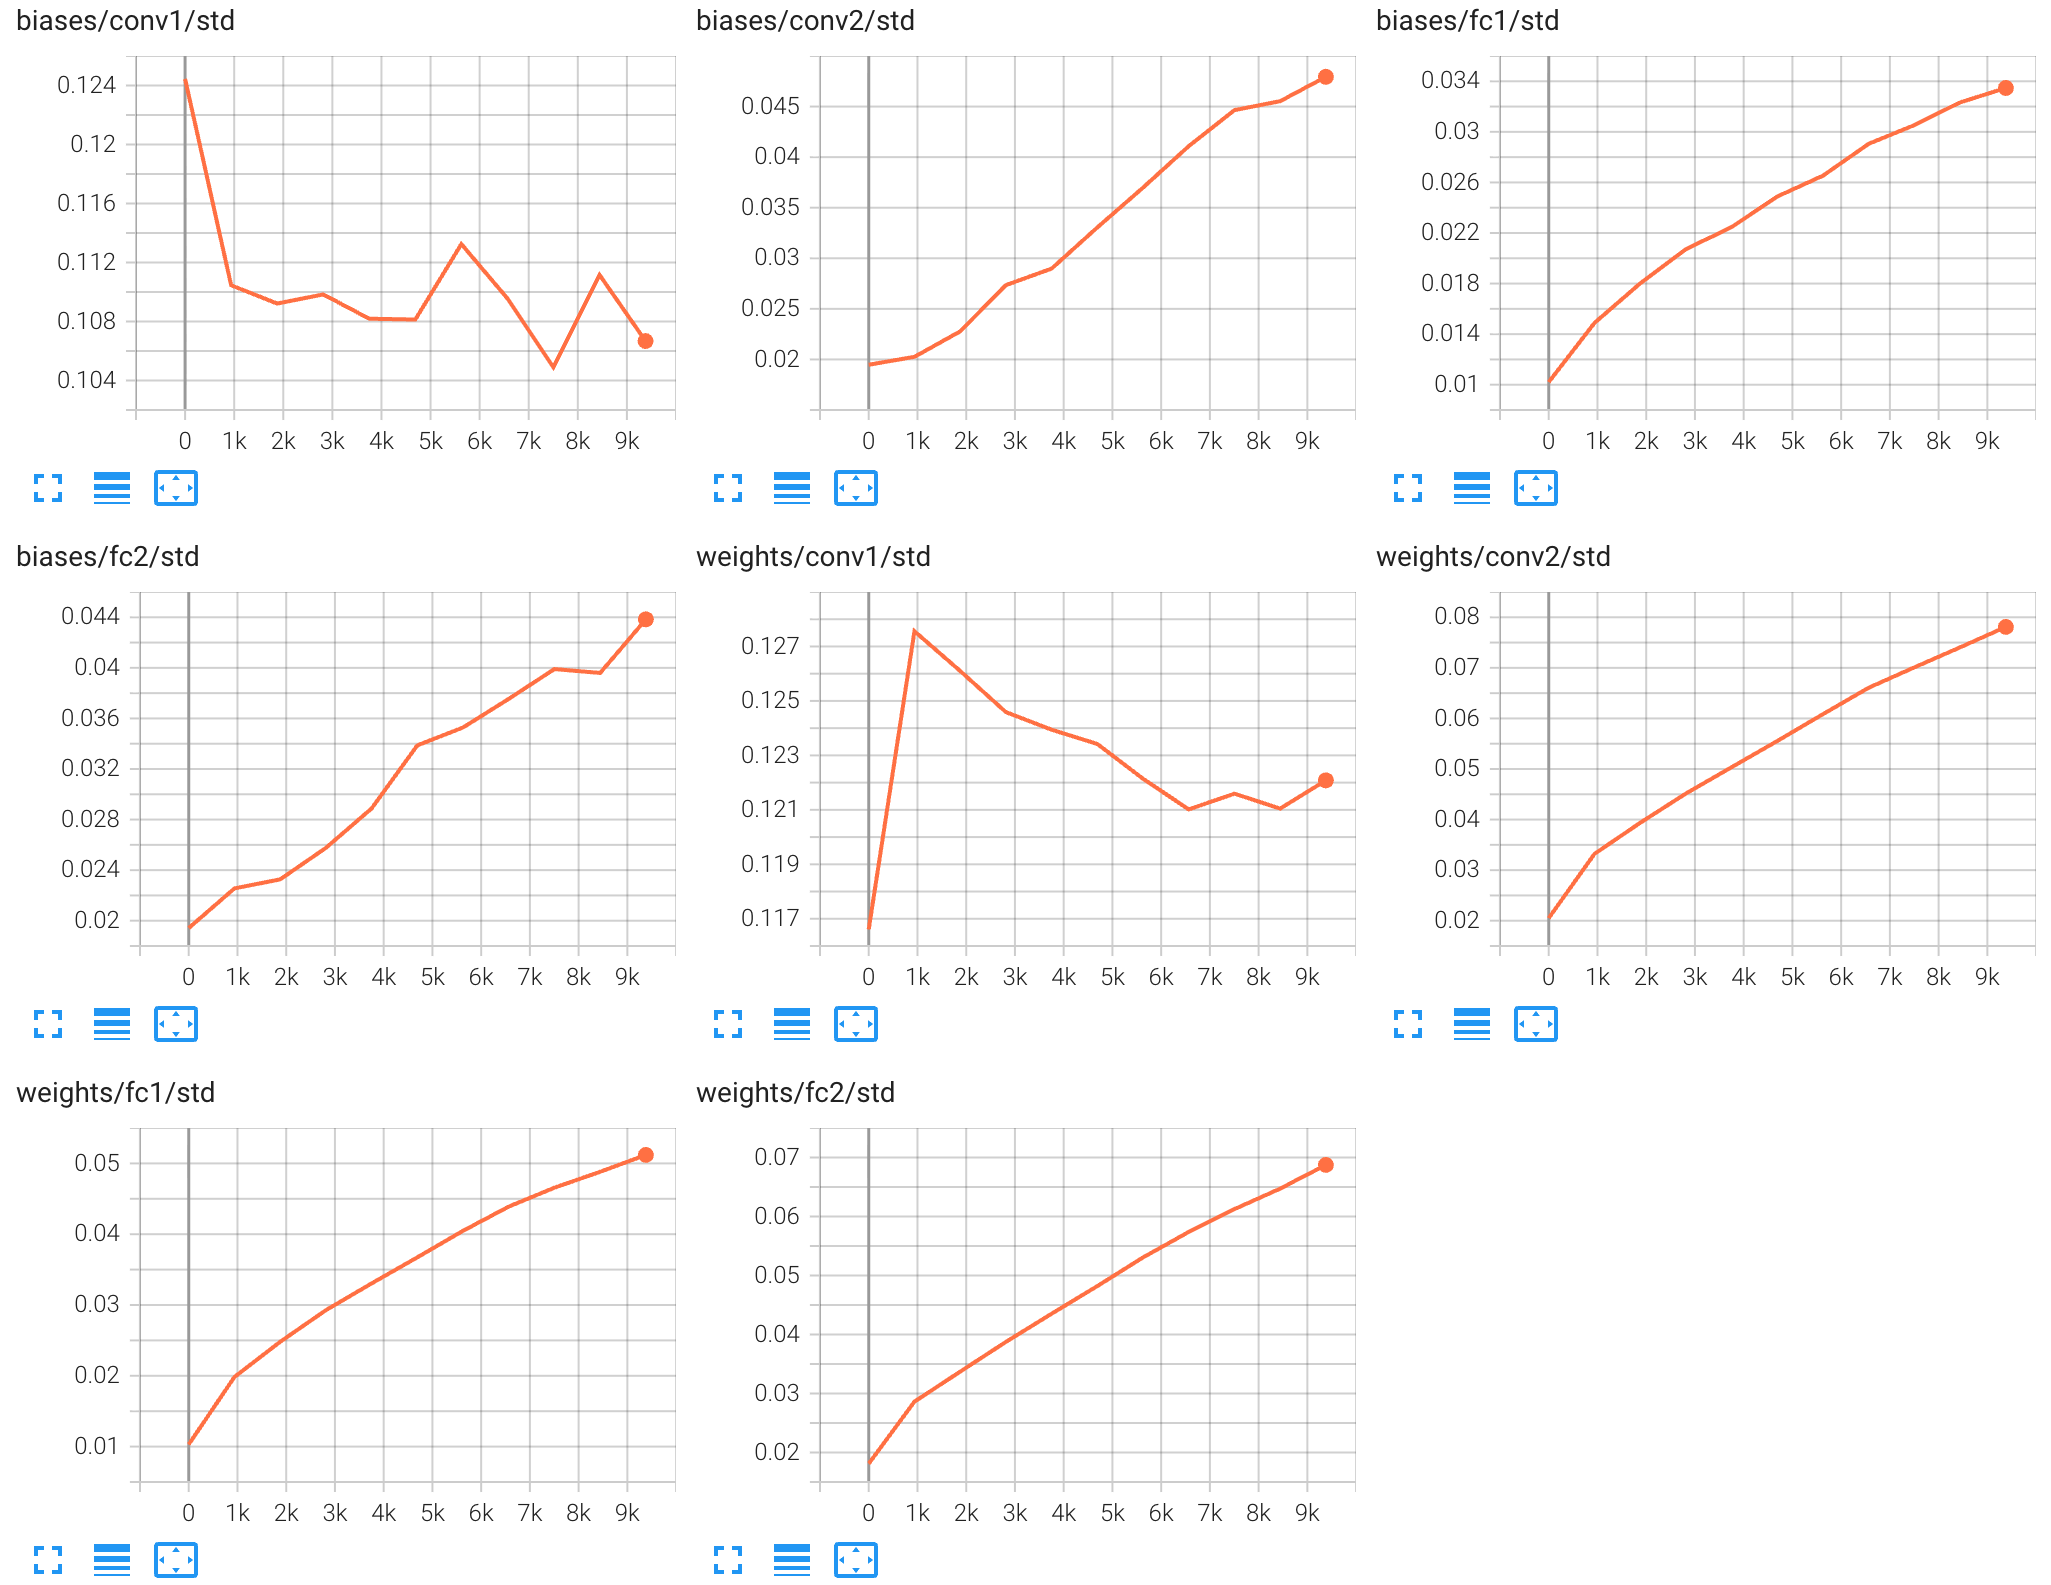
\includegraphics[width=0.62\linewidth]{screenshots/b_std_params.png}

\vspace{4pt}
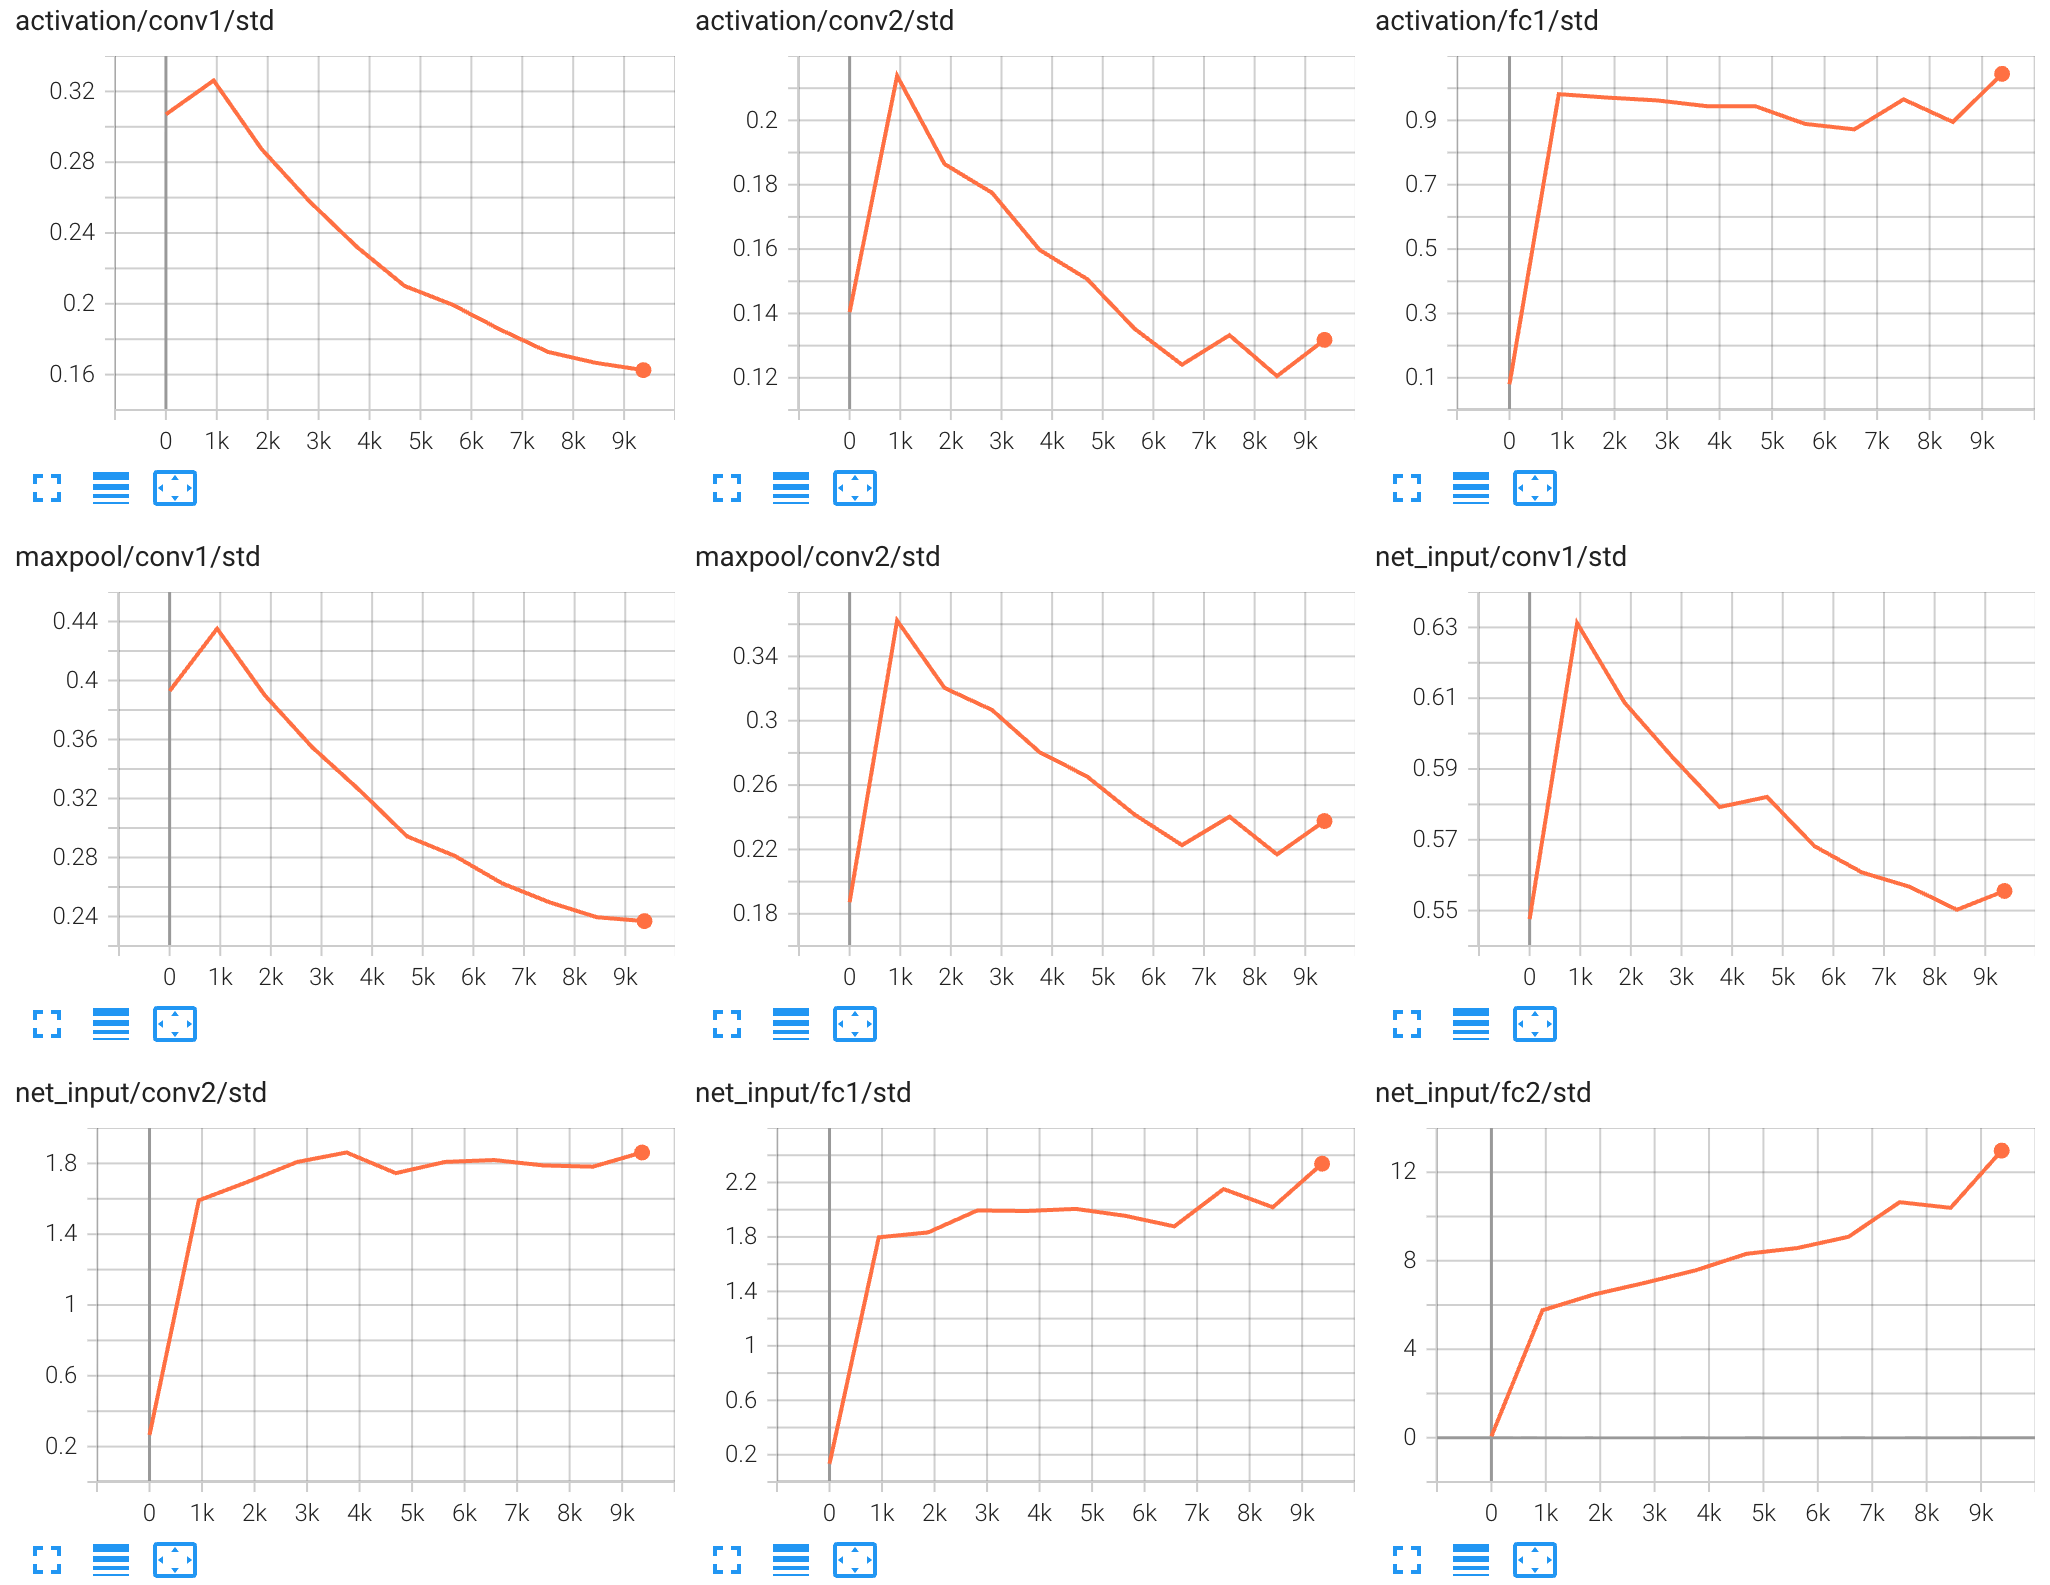
\includegraphics[width=0.62\linewidth]{screenshots/b_std_tensors.png}
\caption{Standard deviation per epoch of every weight and bias (top) and of every net input, ReLU output and max-pool output (bottom).}
\label{fig:bstd}
\end{figure}

Test error drops from 1.20\% after epoch 1 to 0.82\% after epoch 2 and then fluctuates between 0.68\% and 0.92\%. Test loss is lowest at epoch 7 (0.025) and rises to 0.035 by epoch 10, a mild sign of overfitting. The weights spread out during training: the standard deviation of fc1 grows from 0.010 at initialization to 0.051 and is still rising at epoch 10, though more slowly. The fc1 biases drift negative (mean $-0.032$), which turns more fc1 units off. The convolutional activations become sparser over training. The mean conv2 net input moves from $-0.04$ to $-2.14$, and the mean ReLU output of conv2 falls from 0.078 to 0.013, so most conv2 units are zero for any given input and a few respond strongly (max $\approx 7$). The histograms show the same thing: a spike at zero with a long right tail. Max-pooling keeps the largest of four values, so its outputs have two to three times the mean of the ReLU outputs and a thinner spike at zero.

\subsection{MNIST: Activations, Initialization and Optimizers}

Table~\ref{tab:mnist} lists all runs. The activation runs change only the nonlinearity (Adam, $10^{-3}$, default PyTorch initialization). The initialization runs use plain SGD (lr 0.01), where the starting scale matters more than under Adam. Xavier is uniform Glorot; Kaiming is He-normal for ReLU; biases are set to zero in both. The optimizer runs use ReLU and default initialization.

\begin{table}[H]
\centering
\caption{MNIST test accuracy (\%), 10 epochs.}
\label{tab:mnist}
\begin{tabular}{llllcc}
\toprule
Run & Activation & Init & Optimizer (lr) & Epoch 1 & Epoch 10\\
\midrule
baseline & ReLU & default & Adam ($10^{-3}$) & 98.80 & 99.17\\
act\_tanh & tanh & default & Adam ($10^{-3}$) & 98.61 & 98.89\\
act\_sigmoid & sigmoid & default & Adam ($10^{-3}$) & 97.51 & 99.04\\
act\_leaky\_relu & leaky ReLU (0.01) & default & Adam ($10^{-3}$) & 98.58 & \textbf{99.31}\\
\midrule
sgd & ReLU & default & SGD (0.01) & 96.17 & 99.01\\
sgd\_xavier & ReLU & Xavier & SGD (0.01) & 96.69 & 98.97\\
sgd\_kaiming & ReLU & Kaiming & SGD (0.01) & 97.67 & 99.14\\
\midrule
momentum & ReLU & default & SGD+momentum 0.9 (0.01) & 98.50 & 99.14\\
adagrad & ReLU & default & Adagrad (0.01) & 98.44 & 99.20\\
adam\_lr1e-2 & ReLU & default & Adam (0.01) & 11.35 & 11.35\\
\bottomrule
\end{tabular}
\end{table}

\begin{figure}[tbp]
\centering
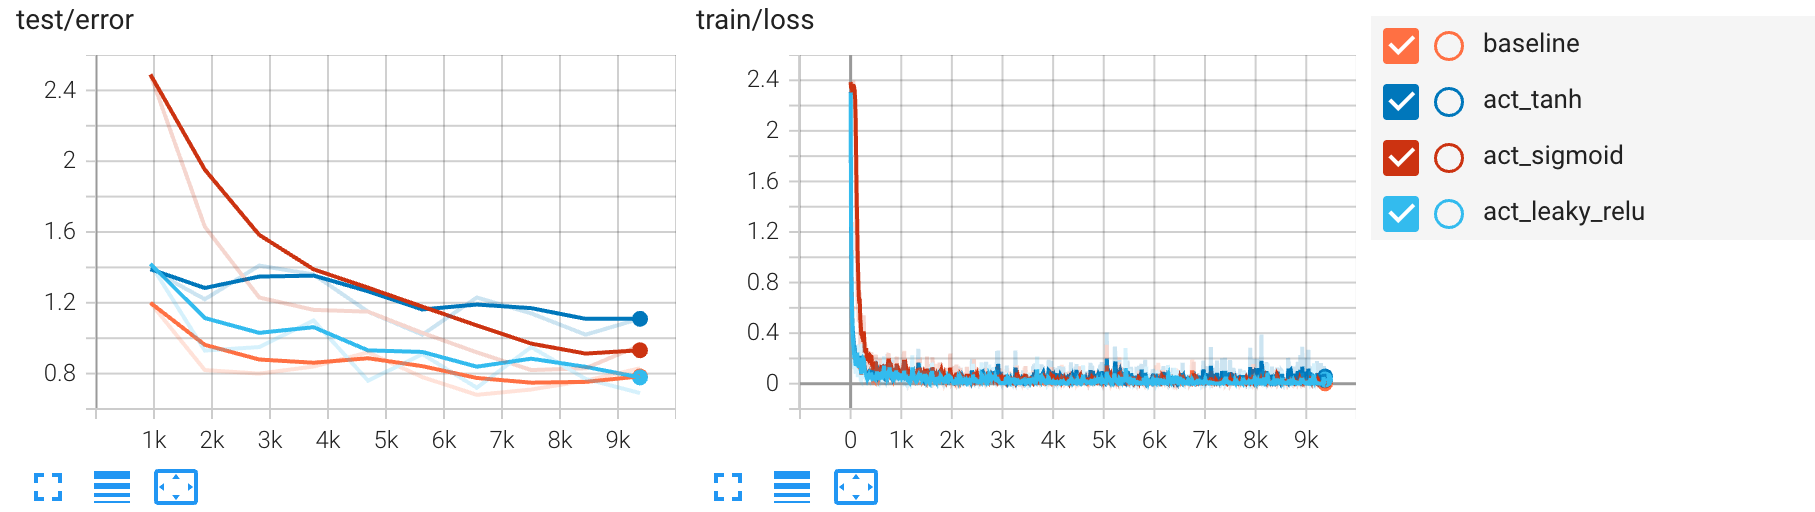
\includegraphics[width=0.85\linewidth]{screenshots/c_act.png}

\vspace{4pt}
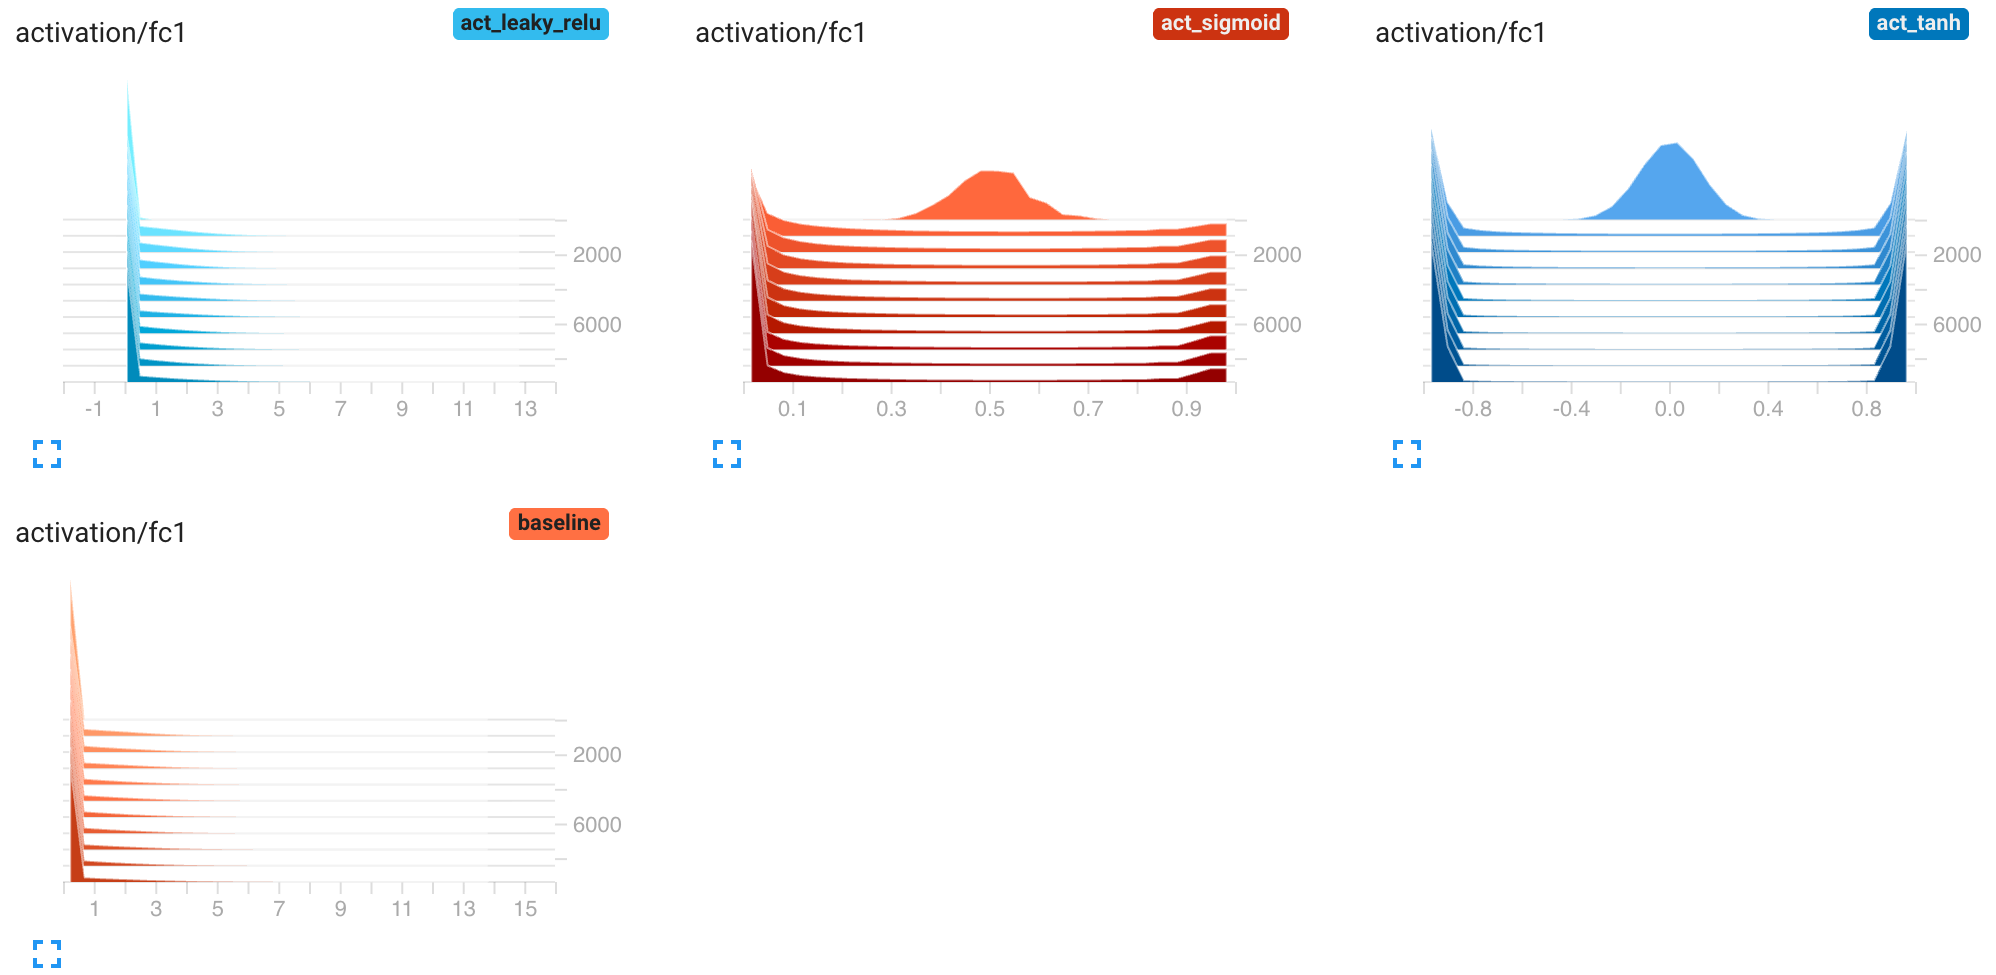
\includegraphics[width=0.75\linewidth]{screenshots/c_act_hist.png}
\caption{Activation functions: test error and training loss (top); histograms of fc1 activations (bottom). Bold curves use TensorBoard smoothing 0.6; faint curves are the raw values.}
\label{fig:cact}
\end{figure}

\textbf{Activations.} All four functions reach 98.9--99.3\%. Leaky ReLU is best and tanh is worst. Sigmoid starts slowest (97.51\% after epoch 1) and is within 0.25\% of ReLU from epoch 7 on. The fc1 histograms in Figure~\ref{fig:cact} show why the squashing functions behave differently. At initialization, the sigmoid and tanh activations sit in a narrow band around 0.5 and 0 (std 0.07 and 0.12). By the end of training most units are saturated, with mass piled at 0 and 1 for sigmoid and at $\pm1$ for tanh (std 0.36 and 0.98). Saturated units pass almost no gradient. Adam's per-parameter scaling compensates enough for the network to train, but tanh's test error stays at 1.0--1.4\% from epoch 2 on. ReLU and leaky ReLU do not saturate on the positive side and produce sparse activations; their histograms are nearly identical, since a slope of 0.01 for negative inputs barely changes the forward pass.

\begin{figure}[tbp]
\centering
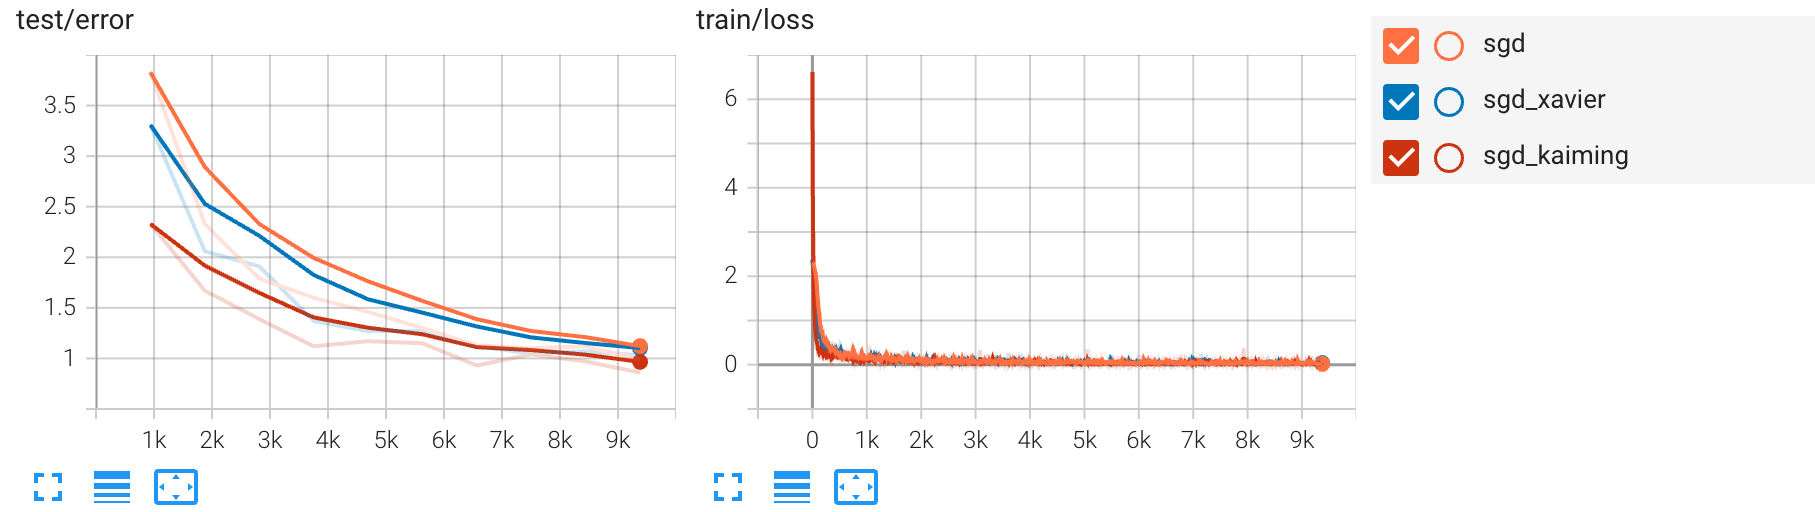
\includegraphics[width=0.85\linewidth]{screenshots/c_init.png}

\vspace{4pt}
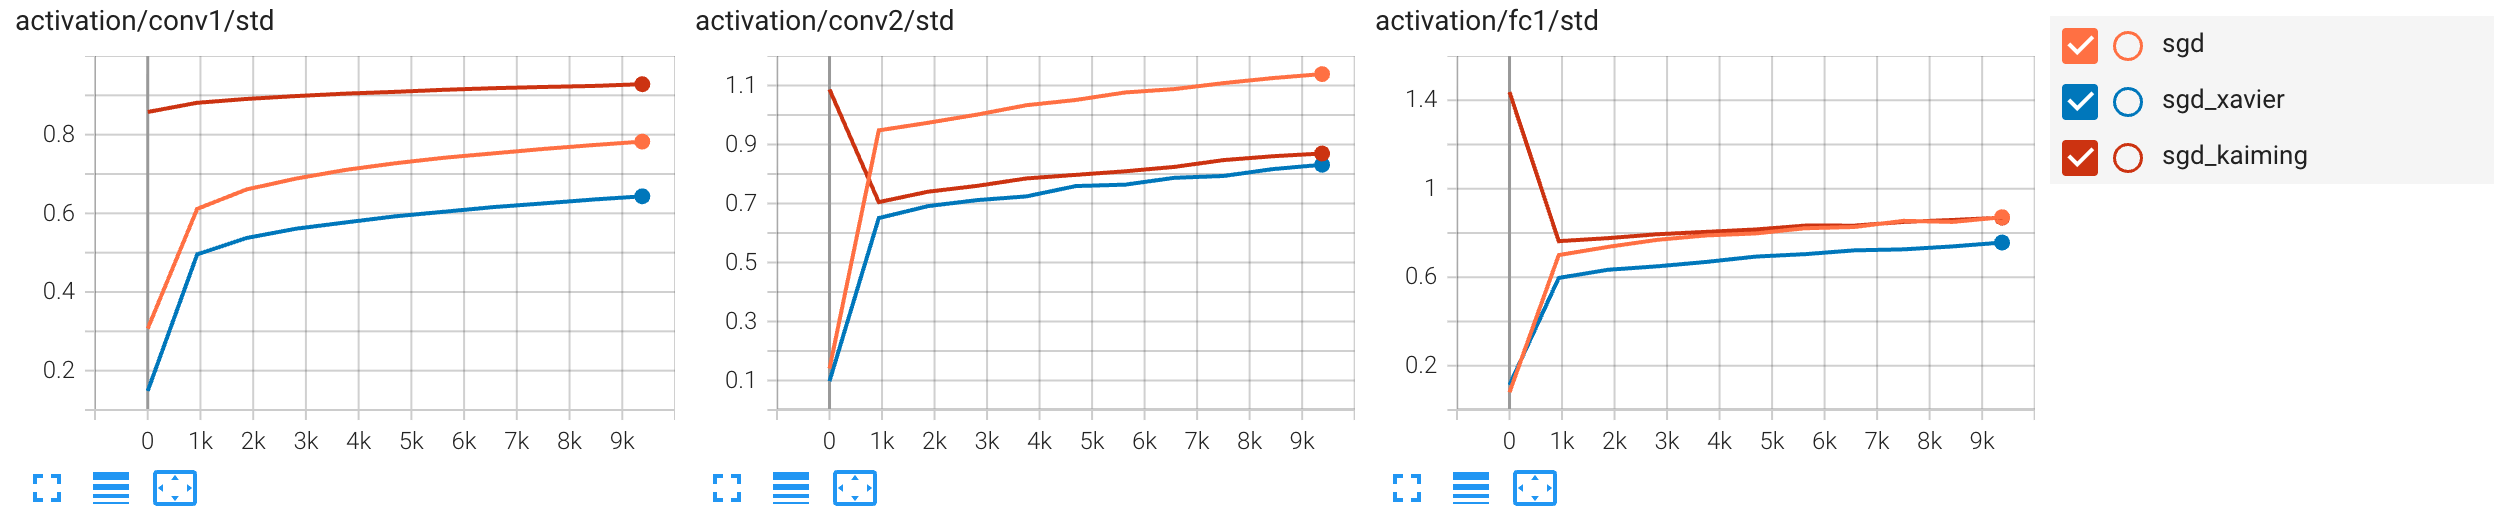
\includegraphics[width=0.95\linewidth]{screenshots/c_init_std.png}
\caption{Initialization under SGD: test error and training loss, smoothing 0.6 with raw values faint (top); std of the ReLU outputs per layer (bottom).}
\label{fig:cinit}
\end{figure}

\textbf{Initialization.} Under plain SGD the initial activation scale determines how quickly the network starts learning (Figure~\ref{fig:cinit}). PyTorch's default (Kaiming-uniform with $a=\sqrt5$, i.e.\ weights in $\pm1/\sqrt{\text{fan-in}}$) and Xavier both start with small activations: the per-layer std of the ReLU outputs at initialization is 0.08--0.31 for default and 0.10--0.15 for Xavier. He initialization preserves the variance through ReLU layers, and its activations stay at order 1 (0.86, 1.09, 1.44 for conv1, conv2, fc1). It reaches 97.67\% after one epoch against 96.17\% (default) and 96.69\% (Xavier), and it finishes highest, at 99.14\%. The cost is an initial training loss of 6.6 instead of 2.3: the ReLU gain is also applied to the linear output layer fc2, so the initial logits are large and the softmax starts confident and wrong. SGD recovers from this within a few dozen iterations.

\begin{figure}[tbp]
\centering
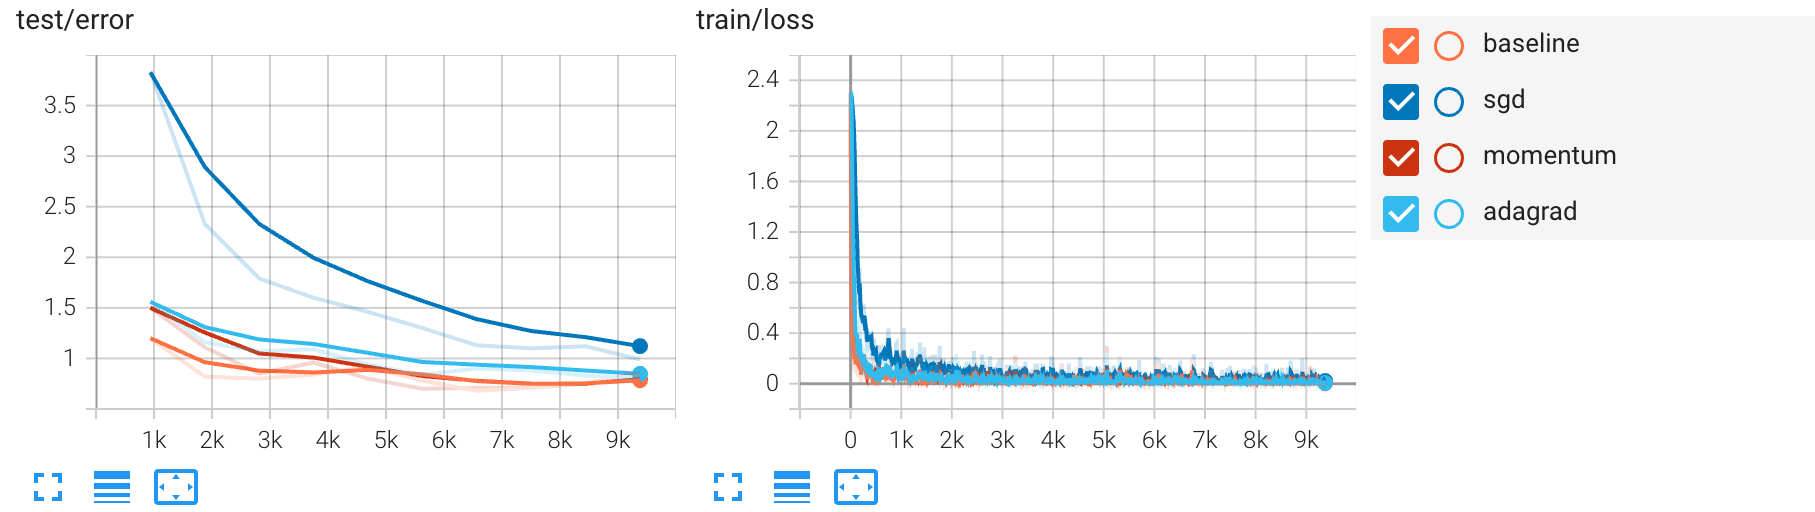
\includegraphics[width=0.85\linewidth]{screenshots/c_opt.png}
\caption{Optimizers: test error and training loss. Smoothing 0.6, raw values faint. Adam with lr 0.01 is left out because its 88.65\% test error flattens the scale.}
\label{fig:copt}
\end{figure}

\textbf{Optimizers.} With a working learning rate, all four optimizers end within 0.2\% of each other (99.01--99.20\%). They differ mainly in speed (Figure~\ref{fig:copt}): Adam leads after one epoch (98.80\%), momentum and Adagrad are close behind, and plain SGD needs 7 epochs to reach the error that Adam has after one. In the Adam run with lr 0.01, Adam's update size is roughly lr per parameter regardless of the gradient's magnitude, so in the first steps every fc1 weight moves by about 0.01, against an initial std of 0.010. The fc1 weight std jumps to 0.054 within the first epoch, the pre-activations of conv2 and fc1 are pushed negative everywhere, and all of those ReLUs die (max activation exactly 0 from epoch 1 on). A dead ReLU has zero gradient, so the network cannot recover, and only the fc2 bias keeps learning, which yields a constant prediction.

\subsection{Discussion}

Depth with sigmoid stalls in both parts. A 10-layer sigmoid network on Moons and a 6-layer sigmoid network on Digits barely train, because $\sigma'\le 0.25$ shrinks the gradient at every layer; tanh and ReLU networks of the same depth train normally. On MNIST, sigmoid and tanh units end up saturated, and ReLU units die when the Adam step is too large (lr 0.01). Under plain SGD, He initialization gives the fastest start. With a working learning rate, SGD, momentum, Adagrad and Adam all finish at 99.0--99.2\%, and all working MNIST runs at 98.9--99.3\%.

On the small datasets, extra capacity fits noise. Make-Moons needs 3--4 tanh units, and wider or deeper networks add islands and protrusions around single points, lowering test accuracy from 0.967 to about 0.95. On Digits, one hidden layer already reaches 97--98\%. ReLU boundaries are piecewise linear (Figures~\ref{fig:e1} and~\ref{fig:depth}). In the DCN, conv2 net inputs drift negative during training, so most conv2 units are off for a given image and a few respond strongly.

\medskip
\noindent LLM assistance (Claude) was used for this assignment, as permitted on the Canvas assignment page for graduate students with prior research experience. Code and TensorBoard logs are in the attached \texttt{sj186-assignment1.zip}.

\end{document}
